
%=============================================================================
%  File:          main.tex
%  Author:       Roman Patscheider und Fabian Hilti
%                Automatik Control Lab, ETH Zurich, Switzerland
%                
%  Content:      Template for student reports
%  Creation:     11 Jan 2001
%  Last change:  continuous ...
%=============================================================================
\newif\ifpdf
\ifx\pdfoutput\undefined
  \pdffalse
\else
  \pdfoutput=1
  \pdftrue
\fi

\ifpdf
\documentclass[11pt,            % 11pt Font
               a4paper,         % a4-Paperformat
               twoside,         % twoside
               fleqn,           % Equations appear flush left
               pdftex
               ]{report}
\else
\documentclass[11pt,            % 11pt Font
               a4paper,         % a4-Paperformat
               twoside,         % twoside
               fleqn,           % Equations appear flush left
               openright        % Chapters begin on odd (right) page
              ]{report}
\fi


\ifpdf
     \usepackage[colorlinks,hyperindex]{hyperref}% generates colored links
                                                 % in pdf file
     \usepackage[pdftex]{graphicx}
     \DeclareGraphicsExtensions{.png, .jpg, .pdf}
     \graphicspath{{pictures/}}
\else
     \usepackage[dvips]{graphicx}
     \DeclareGraphicsExtensions{.eps}
     \graphicspath{{pictures/}}
\fi

\usepackage[T1]{fontenc}        % T1-Fontcoding, auch notwendig
                                % um mit Umlauten ,, arbeiten zu koennen
\usepackage{ae}                 % Almost european computer modern font
                                % Zur Erstellung von pdf-Files
\usepackage[english]{babel}      % Package for multilingual style options
\usepackage{fancyhdr}           % Package for customizing page layout
\usepackage{ETHkopfTwo}         % ETH Style Title page
\usepackage{AufgTwo}            % Formatiert die Aufgabenstellung
\usepackage{verbatim}           % Package for including files
\usepackage[final]{pdfpages}	% Bindet PDF ein
\usepackage{amsmath}

%=============================================================================
% Layout Header and Footer
%=============================================================================

\pagestyle{fancy}
% with this we ensure that the chapter and section
% headings are in lowercase.
\renewcommand{\chaptermark}[1]{\markboth{\thechapter\ #1}{}}
\renewcommand{\sectionmark}[1]{\markright{\thesection\ #1}}
\fancyhf{}                           % Delete all current settings
                                     % for header and footer
\fancyhead[LE,RO]{\bfseries\thepage} % Pagenumber aligned left on odd pages
                                     % Pagenumber aligned right on
                                     % even pages
\fancyhead[LO]{\nouppercase{\bfseries\rightmark}}
\fancyhead[RE]{\nouppercase{\bfseries\leftmark}}
\renewcommand{\headrulewidth}{0.5pt}
\renewcommand{\footrulewidth}{0pt}
\addtolength{\headheight}{1.6pt}     % Make space for headrule
\fancypagestyle{plain}
{
\fancyhead{}                         % Get rid of headers on plain pages
\renewcommand{\headrulewidth}{0pt}   % Get rid of headerline on plain pages
}

%=============================================================================
% Pagelayout
%=============================================================================

\addtolength{\headwidth}{1.2cm}
\addtolength{\textwidth}{1.2cm}
\addtolength{\evensidemargin}{-1.2cm}
\addtolength{\oddsidemargin}{-0cm}


%=============================================================================
% Numbering depth for headings
%=============================================================================
\setcounter{secnumdepth}{3} % Within document
\setcounter{tocdepth}{3}    % Within table of contents

%=============================================================================
% New commands
%=============================================================================

% These commands may be used instead of the built-in commands of LaTeX
% for creating your equations
\newcommand{\be}{\begin{equation}}          % Abbreviation
\newcommand{\ee}{\end{equation}}
\newcommand{\bea}{\begin{eqnarray}}
\newcommand{\eea}{\end{eqnarray}}


%Command clear used to produce empty page without header and footer
%in case of a twoside report where new chapters always begin on odd pages
\ifpdf
   \newcommand{\clear}{}
\else
   \newcommand{\clear}{\newpage{\pagestyle{empty}\cleardoublepage}}
\fi


\frenchspacing

%=============================================================================
% Begin of document
%=============================================================================

\begin{document}
    
\begin{titlepage}
   \pagestyle{empty}
   \topmargin=1.2cm
   \ETHkopfTwo{Automatic Control Laboratory}{Prof. Roy Smith}{Springterm 2012}
   \noindent
   \rule{\textwidth}{0 mm}\\



\begin{center}
\Large \bfseries Semester Thesis\\
\vspace{1cm}
\Huge \bfseries Sensor Fusion / State Estimation for a Kite Power Plant

\vspace{1cm}



%Titelbild einfgen
\vspace{0.1cm}%Grsse verndern zur Positionierung des Bildes

\includegraphics[width=0.75\textwidth]{pictures/titelbild.jpg}
\end{center}

 \vspace{1cm}

    \noindent
    \rule{\textwidth}{1 mm}\\
    \noindent
    \bfseries \large
    \makebox[0.5\textwidth][l]{\emph{Authors:}}
    \makebox[0.49\textwidth][r]{\emph{Advisers:}}

    \vspace{0.2 cm} \noindent
    \makebox[0.5\textwidth][l]{Roman Patscheider}
    \makebox[0.49\textwidth][r]{Aldo Zgraggen}
    \makebox[0.5\textwidth][l]{Fabian Hilti}
    \makebox[0.49\textwidth][r]{Corey Houle}
    \makebox[0.5\textwidth][l]{}
    \makebox[0.49\textwidth][r]{}
    \makebox[0.5\textwidth][l]{}
    \makebox[0.49\textwidth][r]{}
    \mdseries \normalsize


\end{titlepage}

\clear
    \pagenumbering{roman}

    %\include{Vorwort}
\clear
    \tableofcontents
\clear
    \listoffigures % Creates list of all figures used in document
%\clear
    %\listoftables  % Creates list of all tables inserted
\clear
    \chapter*{Abstract}
\addcontentsline{toc}{chapter}{Abstract}

Bla Bla Bla













\clear


% Split your document e.g. chapterwise and rejoin the chapters
% to a single documentation with the \include-Command
    \pagenumbering{arabic}
    \chapter{Introduction}\label{cha1}
\section{Kite Power in General and the SwissKitePower Project}
At a time when windmills were already quite commonly used for power generation, Miles Loyd came up with the idea to use kites to convert wind energy to electricity.  In 1980 he wrote a seminal paper exploring the possibility of generating electrical power using tethered airfoils, i.e. kites \cite{loyd1980}. He describes his concept as follows:
\begin{quote} A kite's aerodynamic surface converts wind energy into motion of the kite. This motion may be converted into useful
power by driving turbines on the kite or by pulling a load on the ground. [...] Not simply facing into the wind, such kites would fly a closed path downwind from the tether point. The kite's motion would be approximately transverse to the wind, in the same sense that a wind turbine's blade moves transverse to the wind. The crosswind airspeed of a kite with this trajectory is increased above the wind speed by the lift-to-drag ratio L/D. The resultant aerodynamic lift is sufficient to support a kite and to generate power. \cite{loyd1980}\end{quote}
Today, several research groups around the world are investigating this subject and working on prototypes. For example the University of Torino have already tested a prototype \cite{canale2006} and Massimo Ippolito has founded a company named KiteGen that is also located in Torino. At the University of Delft the group of Prof. Dr. Wubbo Oeckels is developing kites to produce energy with "Laddermills" \cite{schmehl2012} and at the K. U. Leuven the group of Prof. Moritz Diehl is working on the Highwind project \cite{geebelen2012}. Furthermore the SkySails company is already using wind power to pull large cargo ships \cite{erhard2012} and Ampyx Power, a spin-off from T.U.Delft is working on their PowerPlane device. These European research efforts are all pursuing the approach where power is generated on the ground. In the United States however, the more popular strategy is to generate the electricity up in the air. Two examples of companies trying to establish this technology are Makani Power \cite{makani} and Joby Energy \cite{joby}.  

In Switzerland the research efforts are coordinated in the SwissKitePower Project \cite{skp}. SwissKitePower is a collaborative research and development project between FHNW (University of Applied Sciences Northwestern Switzerland), ETHZ (Swiss Federal Institute of Technology Zurich), EMPA (Swiss Federal Laboratories for Materials Testing and Research) and Alstom Switzerland AG. The goals of the project are to develop 'novel wind energy extraction technology' using tethered airfoils, or kites, and to promote this innovative new technology to the world.



\section{Motivation and Methods}
To successfully implement an automated control algorithm on a kite, it is essential that a precise and fast position estimation is available. Due to the slow update rate of the GPS units and their limited reliability, a Kalman Filter will be used to integrate IMU measurements, which consist of acceleration, rate of turn and magnetic field, with the GPS position and velocity estimations. A standard Kalman Filter, one that could also be used in an airplane for example, assumes no knowledge aboout forces acting on the body. Such an estimator will already enhance the position estimation from the raw GPS input since it incorporates more measurements.  However, a kite can only move on a restricted surface due to it being thethered to the groundstation. An extended Kalman Filter could take advantage of that knowledge and further improve the estimator's performance. Further integrating an aerodynamical model of the kite could give more information about the forces acting on it and would reduce the estimator's dependency on precise sensor output.  

In order to be able to compare the performance of the different estimators, it is neccessary to know the exact location and orientation of the kite at all times. In practice it is nearly impossible to obtain such a ground truth for a kite flying around in the air. Therefore we decided to investigate the benefits of an accurate physical model on the performance of a Kalman Filter using box suspended by a string. (See chapter \ref{setup}) This setup can be modeled as a spherical pendulum which has the advantage that all the main forces acting on it are known.  In addition, we are able to test the algorithms indoors using a Vicon System\footnote{Vicon is a company that comercially sells Motion Tracking systems. cite{vicon}} that gives us a very accurate ground truth of the box's position and orientation. Since there is obviously no GPS reception indoors, the GPS output needs to be simulated using the Vicon's position output, reducing its frequency and adding an appropriate level of noise.


\section{Related Work}
There are many publications on the topic of IMU/GPS data fusion for navigation purposes. As a starting point of our work we used the Master Thesis of Andr\'{a}s H\'{e}jj "Kalman-filter based position and attitude estimation algorithms for an Inertial Measurement Unit" \cite{hejj}. In an other Master project at the University of Southern Denmark Ushanthan Jeyabalan implemented a Kalman Filter using a spherical pendulum model \cite{ushanthan}.
Several other publications investigated the use of a Kalman Filter for IMU/GPS data fusion in different applications. Sukkarieh applied it to land vehicles \cite{sukkarieh1999}, Kim used it for unmanned areal vehicles in highly dynamic flight situations \cite{kim2006} and Crassidis used a Sigma Point Kalman Filter and compared it to an EKF. This list of course is not exhaustive. A much broader overview over the various approaches to multisensor data fusion in target tracking can be found in the survey article of Smith and Singh \cite{smith2006}.
 




 % TeX includes file Chapter1.tex
\clear
    \chapter{IMUs}\label{cha2}

For estimating the kite's state measurements from different sensors are needed. An inertial measurement unit (IMU) contains several sensors that measure physical quantities like acceleration, rate of turn, a magnetic field or ambient air pressure. There are many different such IMU's available, which may be distinguished by which sensors are embedded, at what rate they provide the data, what is their range and sensitivity and how much signal processing is done internally.

The Swiss Kite Power Project has the following options of IMUs to choose:

\begin{description}
\item[MTi-G]
The MTi-G development kit is a commercial product from the Dutch company Xsens. The unit has an accelerometer, gyroscope, magnetometer, pressure sensor and GPS with antenna included. It exist two output data formats. It can be chosen wether the output is raw data or calibrated data. The calibrated data from the sensors without GPS gives the data in common units and uses a calibration to compensate offsets. In addition, the GPS and IMU data can be processed with an Extended Kalman Filter resulting in a filtered output of position and attitude.

\item[PX4]
The PX4 is a open-source/open-hardware IMU used and developed by the PIXHAWK Project of the Computer Vision and Geometry Lab of ETH Zurich. The unit contains a temperature and pressure sensor, an accelerometer, a gyroscope and a magnetometer. The IMU additionally provides a counter for each sensor to ensure an easy handling of the different output frequencies of the included sensors. The output of the sensors is raw data. In the estimation algorithm (see chapter \ref{cha3}) only the embedded accelerometer a BMA180 from Bosch (see the data sheet in appendix \ref{ds_acc}), the gyroscope a L3GD20 from STMicroelectronics (see the data sheet in appendix \ref {ds_gyro}) and the magnetometer a HMC5883L from Honeywell(see the data sheet in appendix \ref{ds_mag}) are used.

\item[x-IMU]
The x-IMU is a product of the company x-io Technologies. It also has a temperature sensor, an accelerometer, a gyroscope and a magnetometer. The configuration of the x-IMU was done by the FHNW. It provides only raw data. The data sheets of the sensors can be found in the appendix \ref{ds_ximu}.
\end{description}


\section{Centrifuge Test}
There are several performance requirements on an IMU installed on a kite. One of them is the dependency on acceleration because a kite experience acceleration of multiple times g. Therefore a centrifuge test was carried out in corporation with the Fachhochschule Nordwestschweiz (FHNW)
\subsection{Set-up}
The setting of the centrifuge is described in figure \ref{centrifuge}.
\begin{figure}[hb]
\begin{center}
\includegraphics[width=0.8\textwidth]{pictures/centrifuge.JPG}
\caption{Picture of the centrifuge.}
\label{centrifuge}
\end{center}
\end{figure}
It was provided by the FHNW. An arm is rotated by a motor. The IMUs are mounted in a box at the end of the arm. The sensors are put next to each other to have similar measurements in all sensors. A psicture of the Box can be seen in figure \ref{box}. 
\begin{figure}[hb]
\begin{center}
\includegraphics[width=0.8\textwidth]{pictures/box.JPG}
\caption{Picture of the box with the IMUs inside.}
\label{box}
\end{center}
\end{figure}
Obviously, the motion of the box is describing a circle with a radius (the distance between the rotation axis and the  center of the box) of $0.75\;m$. The motor is able to rotate the arm with a velocity of about $10\; m/s$. Which corresponds to a maximum acceleration of about $ a=\omega*r^2=8\;g$. 

Even though a sensor on the centrifuge was measuring the rate of turn, there was no software for the data collection implemented. Therefore we have no ground truth to compare the sensor data with. 
During the test, the motor was driven in order to have 5 steps between $1.62\;g$ and $7.8\;g$ $(ca.\;1.6\;g;\;2.4\;g\;3.7\;g;\;5.4\;g;\;6.9\;g;\;7.8\;g)$ of centripetal acceleration.

The PX4 and MTi-G are connected together. Both, the PX4 and the MTi-G measurements are written on the SD card of the PX4 Unit. The timestamps for the sensor readings are taken from the GPS clock for the MTi-G as well as for the PX4 at the time when they are logged on the SD card. This results in easy and accurate synchronization between the two IMUs. To get the time synchronized with the third IMU, the x-IMU is synchronized to the computer's time. Additionally the 3 sensors are hit for having a clearly distinghuishable signal aiding in the estimation of how accurate the synchronization is.
\FloatBarrier
\subsection{Result}
The raw data from the x-IMU is scaled by Raphael Mueller bringing it to the common units $m/s^2$ for the accelerometer, $deg/s$ for the gyroscope and $gauss$ for the magnetometer.

The PX4 was set by the group of the PixHawk Project. How the output of the sensors have to be scaled to bring them in the required units is shown in table \ref{ct_units_PX4}. The scale factor describes by how much the output has to be multiplied to get the data converted in the units described in 4th row.
\begin{table}[h]
\centering
\begin{tabular}{|p{2.5 cm}|c|c|c|p{3 cm}|}
 \hline
 Sensor & Sensitivity & Scale Factor & Unit & Comment \\
 \hline
 Accelerometer BMA180 & $2048\;LSB/g$ & $output*9.81/2048$ & $m/s^2$ &     Sensitivity range: $+/- 4\;g$ \\
 \hline
 Gyroscope L3GD20 & $17.5\;mdps/digit$ & $output*17.5/1000$ & $deg/s$ &  Sensitivity range $+/- 500\;dps$ \\
 \hline
 Magnetometer HMC5883L & $1370\;LSB/g$ & $output/1370$ & gauss &   Sensitivity range $+/-8\;gauss$\\
\hline
\end {tabular}
\caption{This table shows how the raw data output of the PX4 has to be sclaed to get the right units.}
\label{ct_units_PX4}
\end{table}
The MTi-G has also raw output data but no clear explanation in the data sheet in appendix \ref{ds_mti-g} on how to get to the required units. Therefore, were the MTi-G data scaled to bring it more or less to the same order as the other two IMUs are.
In figure \ref{ct_pos} we can see the plot of the GPS data.
\begin{figure}[hb]
\begin{center}
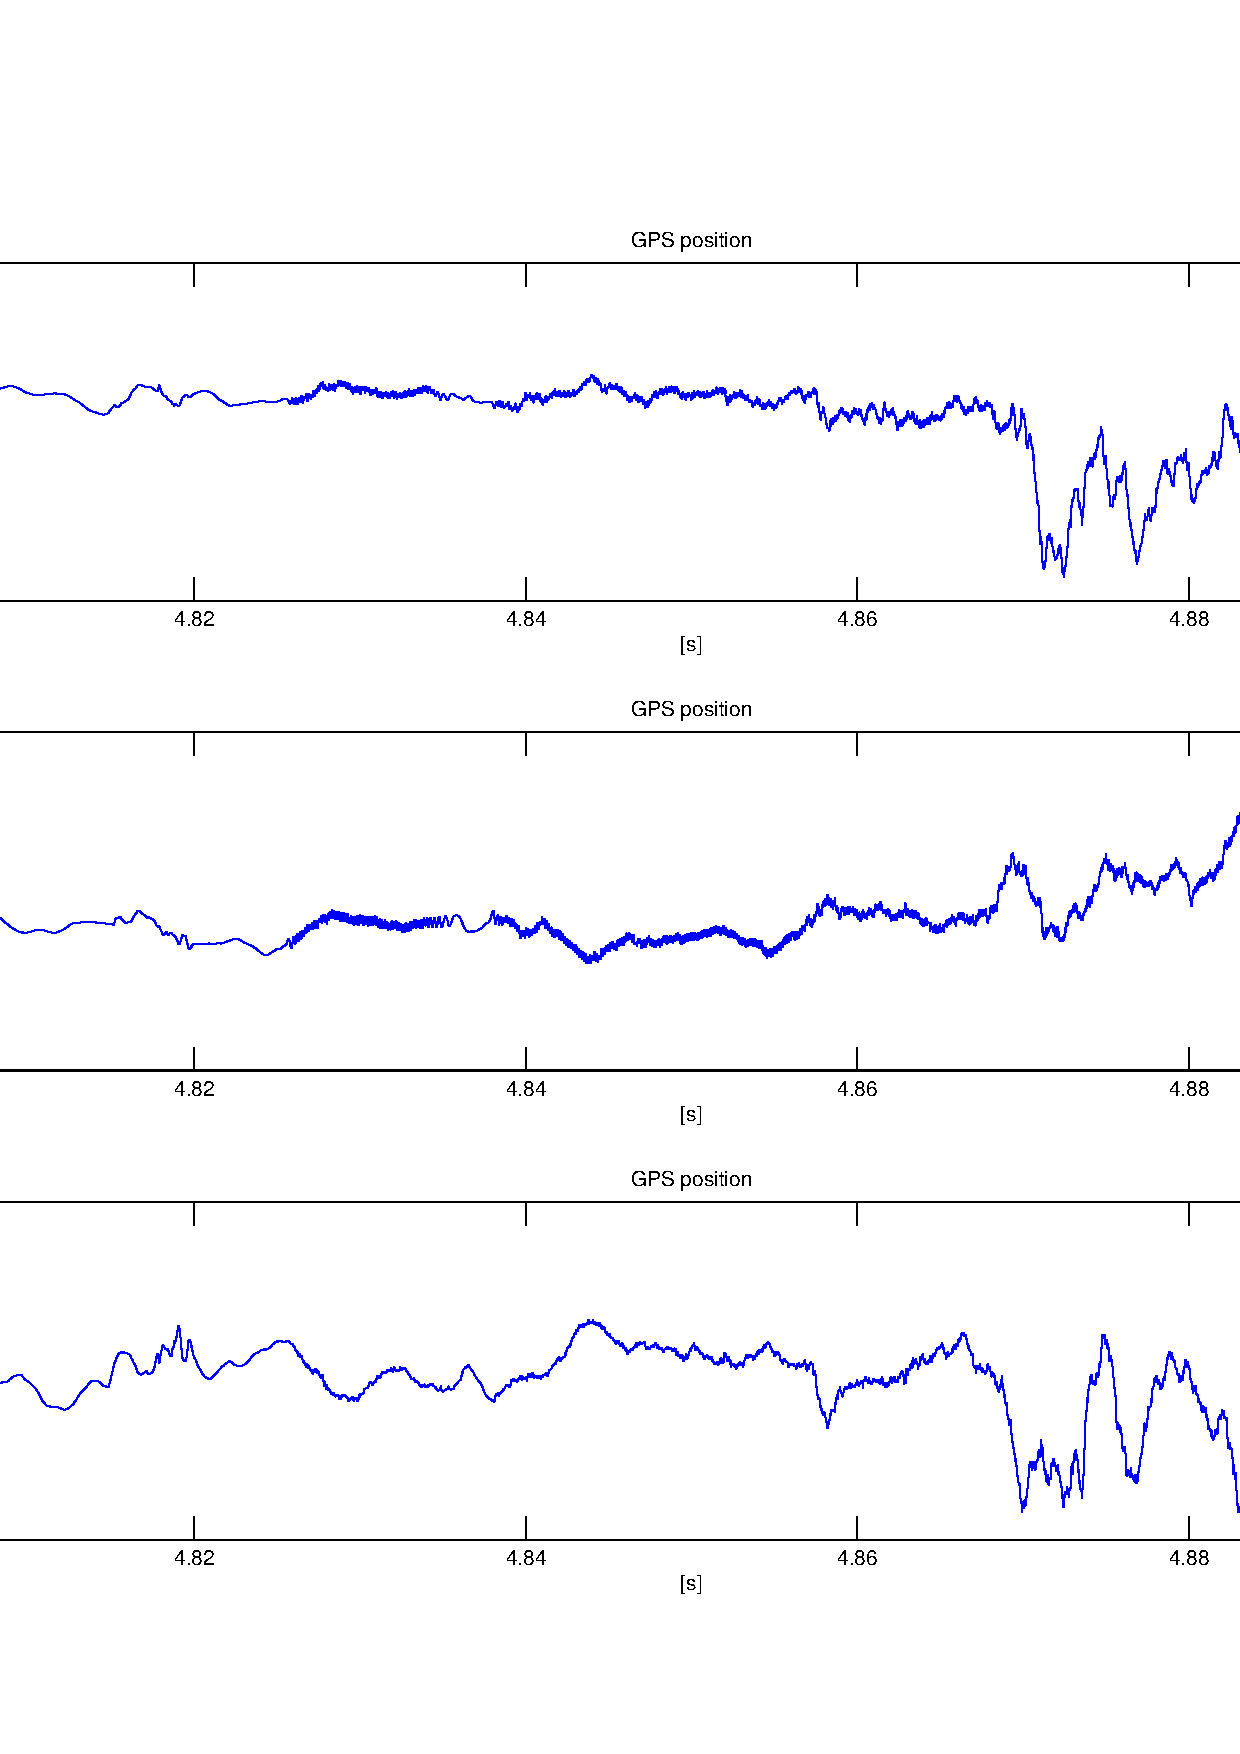
\includegraphics[width=1\textwidth]{pictures/ct_pos.png}
\caption{GPS Position}
\label{ct_pos}
\end{center}
\end{figure}
Until $4.83*10^{4}\; s$ is the centrifuge not in motion. The mean value of this period is taken as the ground truth to calculate the the average error of the GPS signal. The mean value of the north component is $47.48\;deg$ for the east component $8.2138\;deg$ and for the down component $415.74\;m$. The coordinates of Winidsch, where the test takes place is $47.4806\;deg$, $8.2222\;deg$ and $357\;m$. By taking the average absolute difference between the GPS data and the mean value calculated before, an error of the GPS can be estimated: $1.08*10^{-5}\;deg$, $1.37*10^{-5}\;deg$ and $2.49\;m$ for north, east, down respectively. After $4.83*10^{4}\;s$ the noise is increasing. At this time the centrifuge starts rotating. The calculated  errors in this period are: $1.68*10^{-5}\;deg$, $2.27*10^{-5}\;deg$ and $2.89\;m$ for north east and down respectively. After $4.87*10^{4}\;s$ the noise looks even higher. This is when we have  a centripetal acceleration of more than  $6.7\;g$. The estimated noise is: $1.04*10^{-4}\;deg$, $1.02*10^{-4}\;deg$ and $13.01\;m$. Since in non of this periods a cosine of sine behavior of the north and east component can be seen, all three components should be stable in the ideal case. The error values a summarized in table \ref{ct_pos_error}.
\begin{table}[h]
\centering
\begin{tabular}{|l|r|}
\hline
Period & Average error (north/east/down) \\
\hline
$4.80*10^{4}\;s - 4.83*10^{4}\;s$&$1.08*10^{-5}\;deg / 1.37*10^{-5}\;deg / 2.49\;m$\\
\hline
$4.83*10^{4}\;s – 4.87*10^{4}\;s$&$1.68*10^{-5}\;deg / 2.27*10^{-5}\;deg / 2.89\;m$\\
\hline
$4.87*10^{4}\;s – 4.91*10^{4}\;s$&$1.04*10^{-4}\;deg/ 1.02*10^{-4}\;deg / 13.01\;m$\\
\hline
\end{tabular}
\caption{The average error of the postion in different time segments}
\label{ct_pos_error}
\end{table}
Due to the fact that the velocity is the derivative of the position of the GPS the amplitude of the error behaves  similar.
\begin{figure}[hb]
\centering
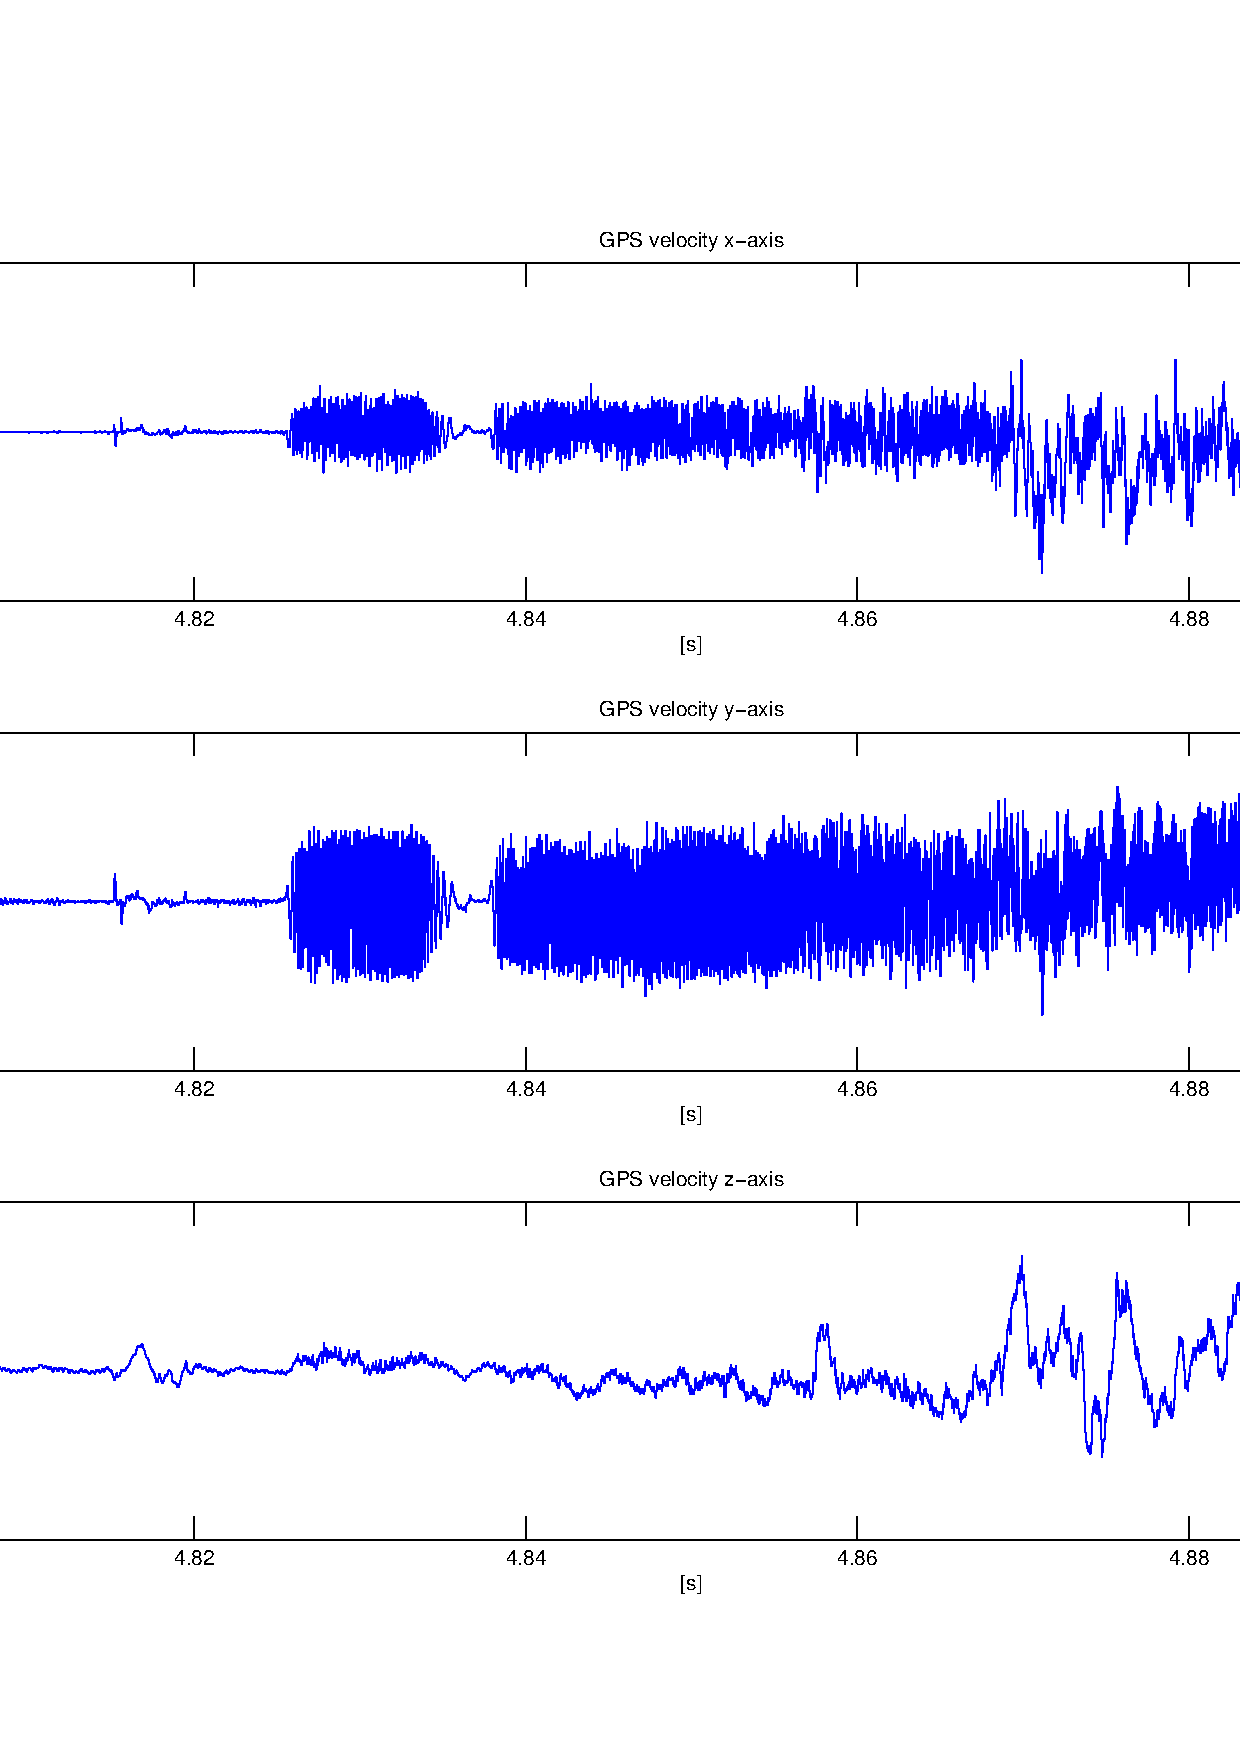
\includegraphics[width=1\textwidth]{pictures/ct_vel.png}
\caption{GPS velocity}
\label{ct_vel}
\end{figure}
The periods with the correspondent average errors is shown in table \ref{ct_vel_error}.
\begin{table}[h]
\centering
\begin{tabular}{|l|r|}
\hline
Period & Average error(x/y/z) \\
\hline
$4.80e4\;s - 4.83e4\;s$&$5.54\;m / 6.05\;m / 6.57\;m$\\
\hline
$4.83e4\;s – 4.87e4\;s$&$101.86\;m / 138.96\;m/ 27.36\;m$\\
\hline
$4.87e4\;s – 4.91e4\;s$&$157.20\;m / 123.56\;m / 58.78\;m$\\
\hline
\end{tabular}
\caption{The average error of the velocity in different time segments}
\label{ct_vel_error}
\end{table}
In figure \ref{ct_acc} and figure \ref{ct_gyro} the accelerometer and gyroscope measurements are shown. 
\begin{figure}[h]
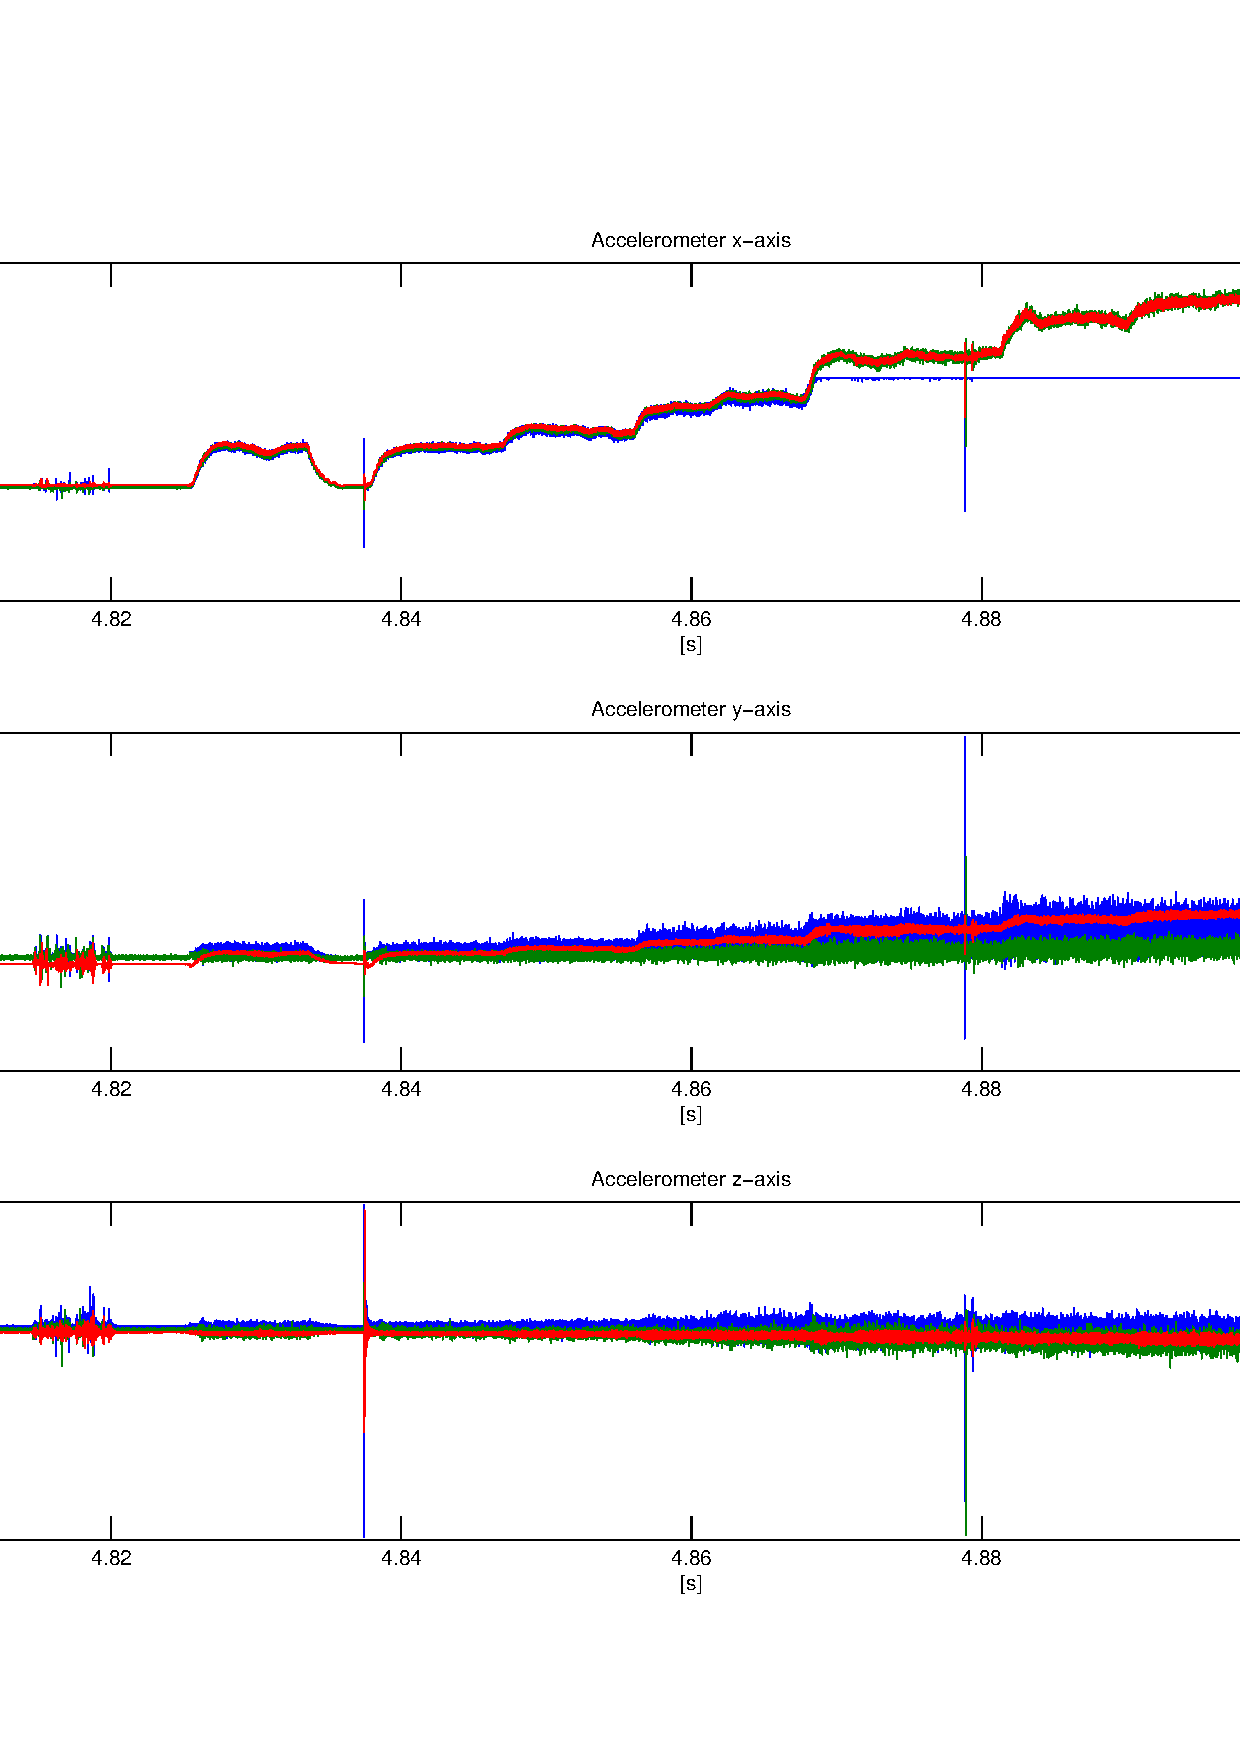
\includegraphics[width=1\textwidth]{pictures/ct_acc.png}
\caption{Accelerometer}
\label{ct_acc}
\end{figure}
\begin{figure}[hb]
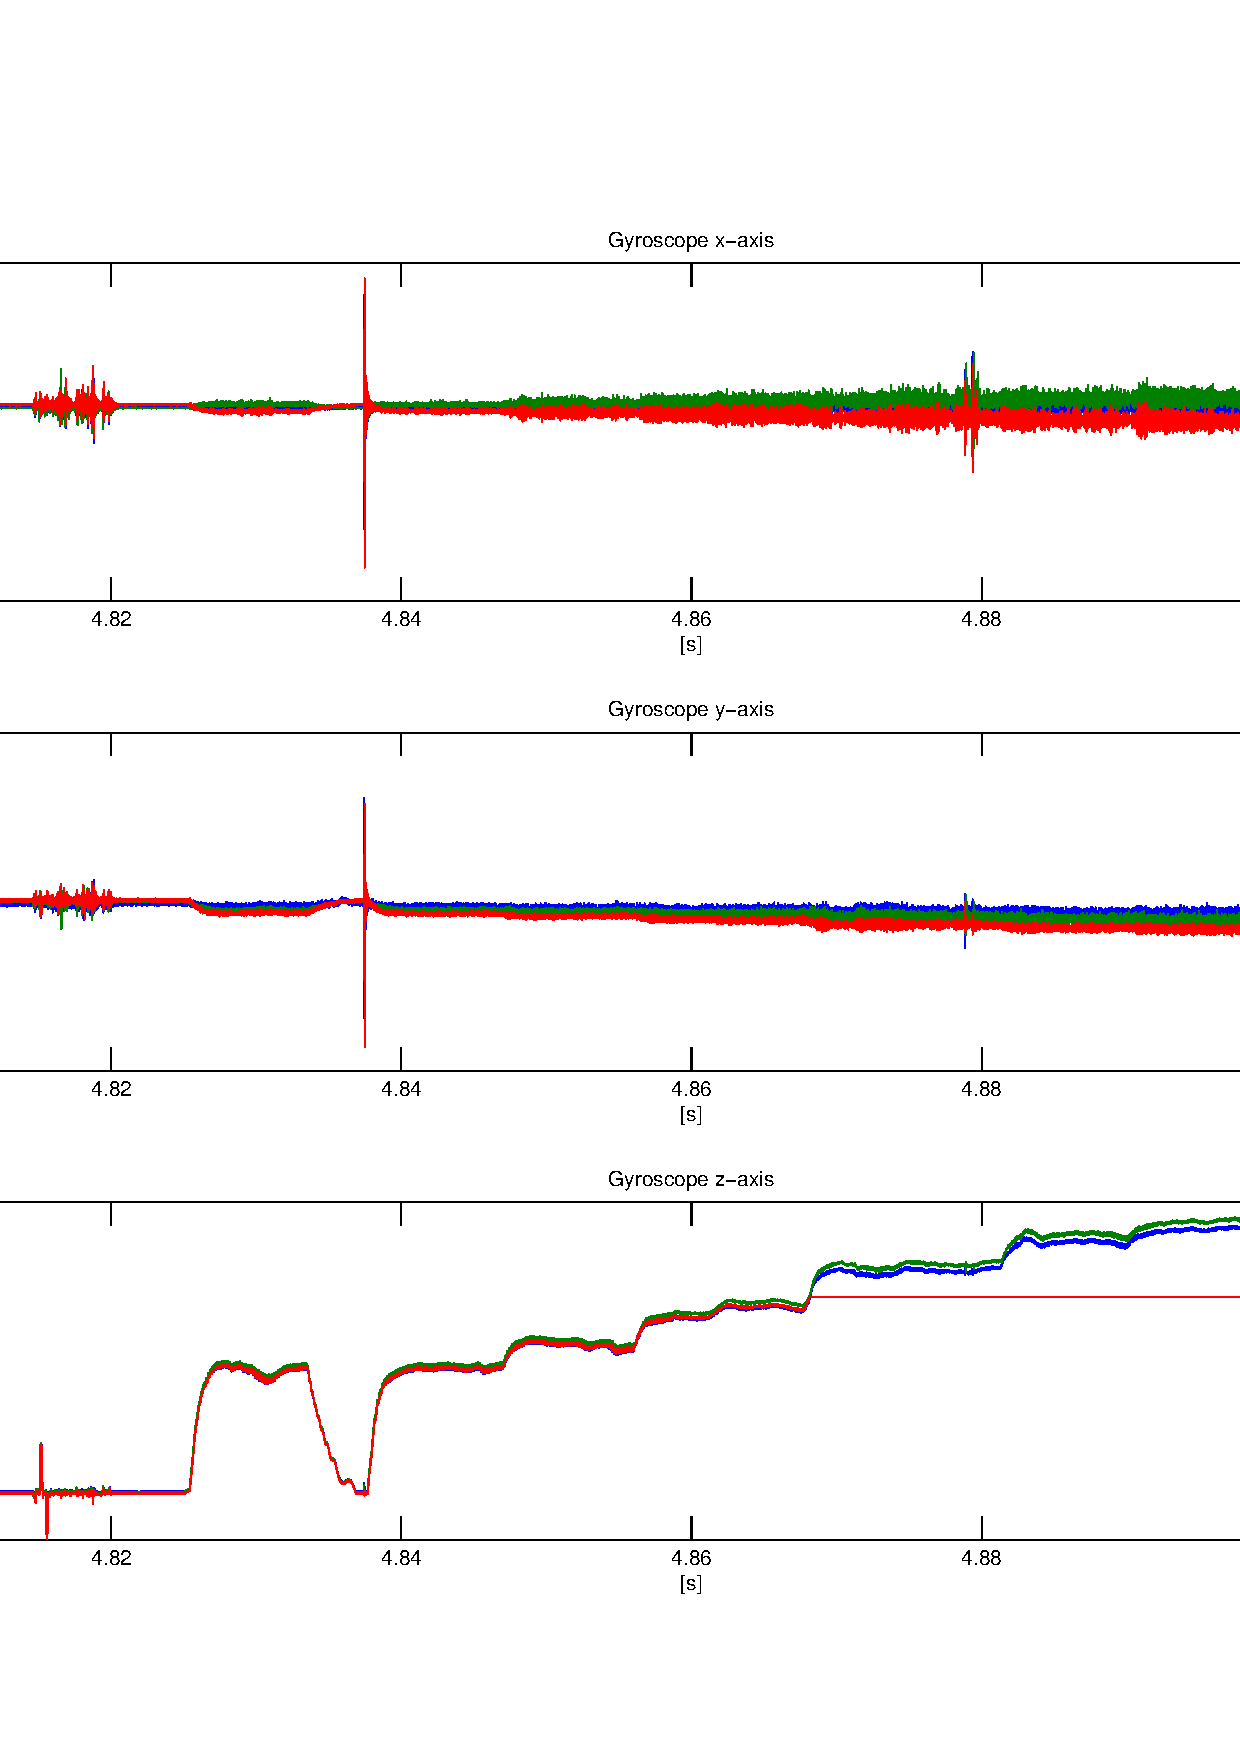
\includegraphics[width=1\textwidth]{pictures/ct_gyro.png}
\caption{Gyrometer}
\label{ct_gyro}
\end{figure}
As expected, we do have the highest acceleration in x direction and the fastest rotational rate in z direction. In the accelerometer x axis and the gyroscope z axis measurements can be seen the 5 steps of different rotational speed. The very first step is a test rotation followed by the hit on the sensors which react with a peak. Since the sensitivity of the PX4 accelerometer is set to $+/- 4 \;g$, the output of accelerometer in x direction is limited to $39.24 \;m/s^2$. The MTi-G Unit is as well limited to $+/- 5\;g$. This is not obviously seen in the plots. The acceleration in y direction is showing small steps which can be accounted for by the placement of the sensors slightly off the center of the box. The gyroscope from the MTi-G shows a limitation in measuring the rate of turn (see figure \ref{ct_gyro}. It is unable to resolve more than $ 403 \;deg/s$. By the choice of the PX4's gyroscope setting the range is limited to $+/- 500\;dps$. But on the plot this limitation is not seen up to $520\;dps$. The x-axis and y-axis should be zero for the gyroscope since the rotation is only two dimensional. Obviously, the noise again increases with higher rates of rotation. This can be clearly seen in the acceleration in z direction which should be constant at $-9.81 \;m/s²$, the gravitation. It looks like the noise level of the PX4 is the highest before the x-IMU and the MTI-G which has the lowest. This can be traced back on the high sensitivity set up of the PX4 accelerometer.


In figure \ref{ct_mag} the magnetometer output is plotted.
\begin{figure}[hb]
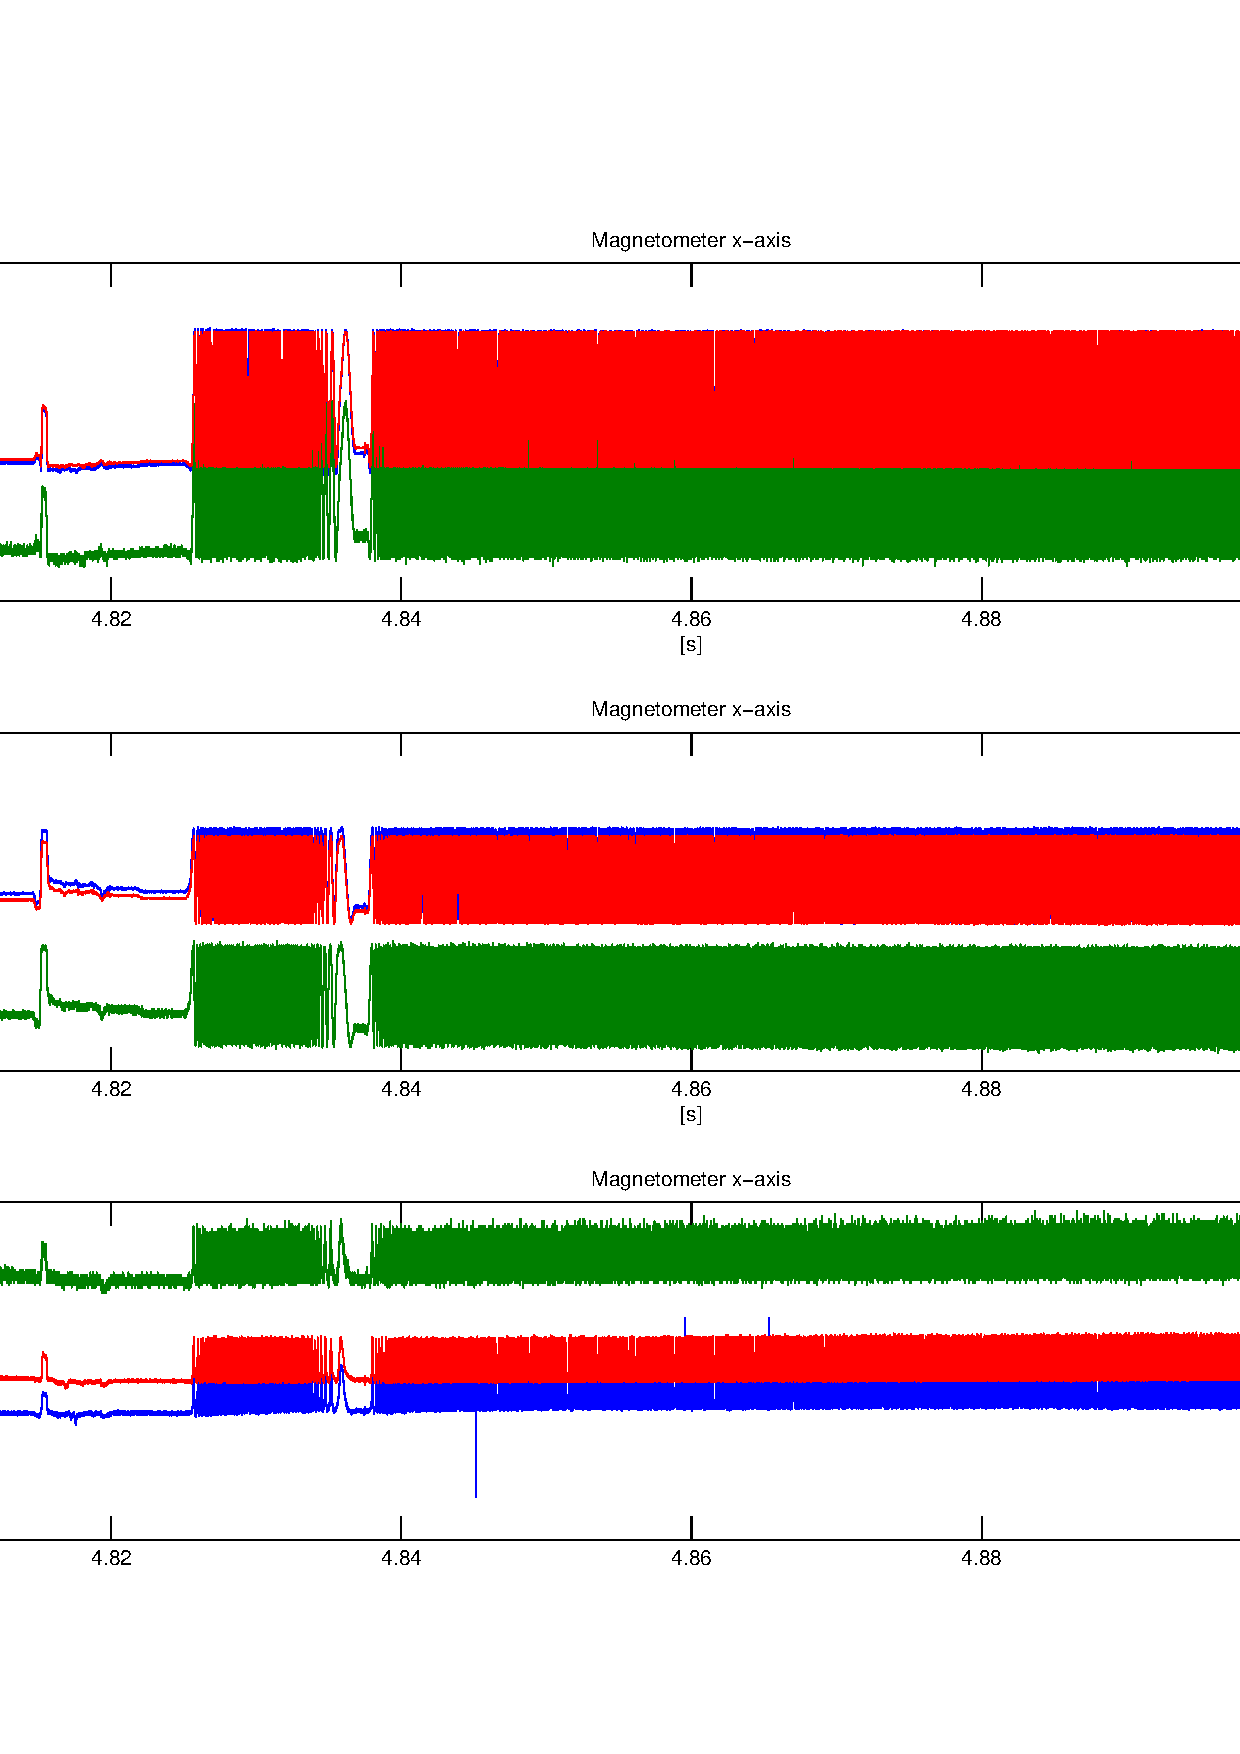
\includegraphics[width=1\textwidth]{pictures/ct_mag.png}
\caption{Magnetometer}
\label{ct_mag}
\end{figure}
There is a misalignment between the x-IMU,MTi-G and the PX4 which cannot be explained by the authors. The range of the maximum value and the minimum value of the PX4, MTi-G and the x-IMU is in x and y direction $0.4 \;gauss$. This is the expected range in the region of Zurich. In this sense, if the the output is added with an offset in order to get the range to $+/- 0.2\; gauss$, the measurements should be correct. The PX4 has a mean value of $0.3893$ gauss while the ground truth is $0.4268 \;gauss$.  The noise of the magnetometer is in the x-IMU higher than in the other two IMUs.The PX4 unit has limited range of $+/-8\;guass$ what not appear in this test and therefor

In figure \ref{ct_sine} a closer look on the x axis of the magnetometer and accelerometer and on the y axis of the gyroscope is presented. The form of the curve has sine behavior, what we would expect again.
\begin{figure}[hb]
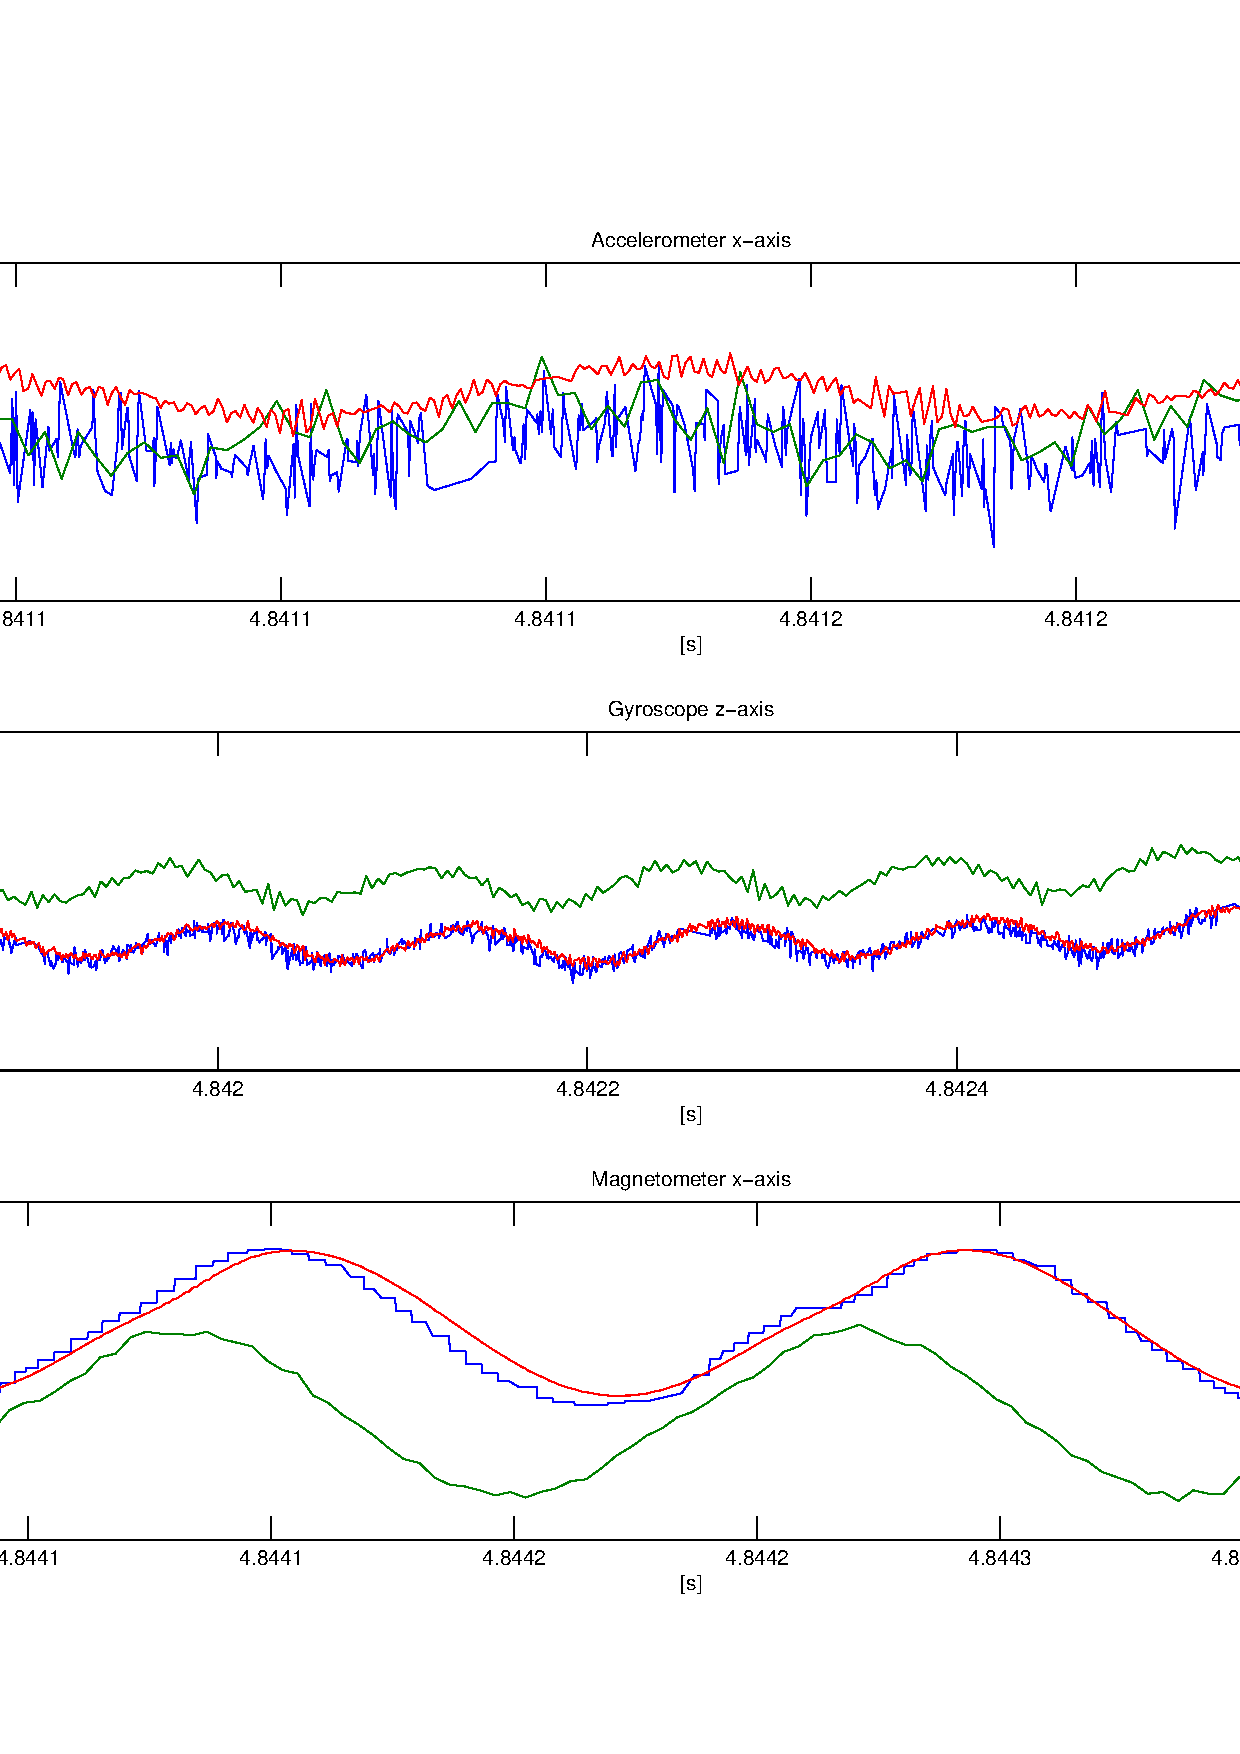
\includegraphics[width=1\textwidth]{pictures/ct_sine.png}
\caption{A closer look in time on the three IMU sensors.}
\label{ct_sine}
\end{figure}

\FloatBarrier
\subsection{Conclusion}
All IMUs work in the same range of noise level. With an increasing rotational velocity and therefore a higher centripetal acceleration, the average error is increasing in all sensors, except in the magnetometer. There could not be found a dependency between noise in the measurement of the magnetic field and the acceleration. 
In a future experiment it would be interesting to also record the rotational rate of the centrifuge in order to have a more accurate ground truth that could be used to determine the accuracy of the IMU measurements. This could lead to a more founded compairison of the the different sensors' accuracy. Finally the sensitivity of the accelerometer of the PX4 unit should be set in a way to be able to observe the whole range of the applied centripetal acceleration and the MTi-G would need to be set to record the data in the calibrated output mode. An arbitrary scaling will then not be necessary anymore.


\clear
    \chapter{State Estimation}\label{cha3}
In this chapter an introduction to the Kalman Filter and the modified version called Extendend Kalman Filter is given. In a second step  the state estimation algorithm, that was developed during this thesis, will be explained. This gives an overview over the whole code and describes how the parameters were set and how a sensor data outage is handled. Sections \ref{state_estimation} and \ref{sensor_estimation} will focus on the two essential parts of the algorithm: The propagation of the states and how the measurements are estimated.


\section{Extended Kalman Filter}

\subsection*{Discrete Kalman Filter}
We will first give a short introduction to the Kalman Filter in general and its mathematical justification.
\begin{quote}The Kalman filter is an extremely effective versatile procedure for combining noisy sensor outputs to estimate the state of a system with uncertain dynamics.\cite{andrews2007}\end{quote} It was published in 1960 by R.E.Kalman. The Filter gained a strong impact in the area of autonomous or assisted navigation \cite{welch1997}. 
Systems in which the filter is estimating the state $x \in R^{n}$ can be described by the following linear stochastic difference equation.
\begin{equation}
x_{k+1}=A_k*x_k+B_k*u_k+w
\label{eq1}
\end{equation} The next equation shows the relation between the state and the measurement $z \in R^{n}$.
\begin{equation} 
z_k=H_k*x_k+D_k*u_k+v
\label{eq2}
\end{equation}
Where the random variables $w$ and $v$ stand for the process and the measurement noise, which are assumed to be independent, white and normal probability distributions.
\begin{equation}
p(w)\sim N(0,Q)\;, \\
p(v)\sim N(0,R)\label{R_Q_noise}
\end{equation}
\begin{quote}The $n\times n$ matrix A in equation \ref{eq1} relates the state at time step $k$ to the state at step $k+1$, in the absene of either a driving function or process noise. The $n\times l$ matrix $B$ relates the control input $u \in R^{l}$ to the state $x$. The $m \times m$ matrix $H$ in the measurement equation \ref{eq2} relates to the state to the measurement $z_k$.\cite{welch1997}\end{quote}
In most navigation applications, the noisy sensors are a GPS receiver and an inertial navigation system or other sensors like for example speed sensors. The states of a system are described by the position, velocity, attitude and attitude rate \cite{andrews2007}.

\subsection*{Mathematical Background}\label{math_kalman}
In figure \ref{simple_schematic} the structure of the algorithm is sketched for a better understanding of the filter's mathematical background. 
\begin{figure}[h]
\begin{center}
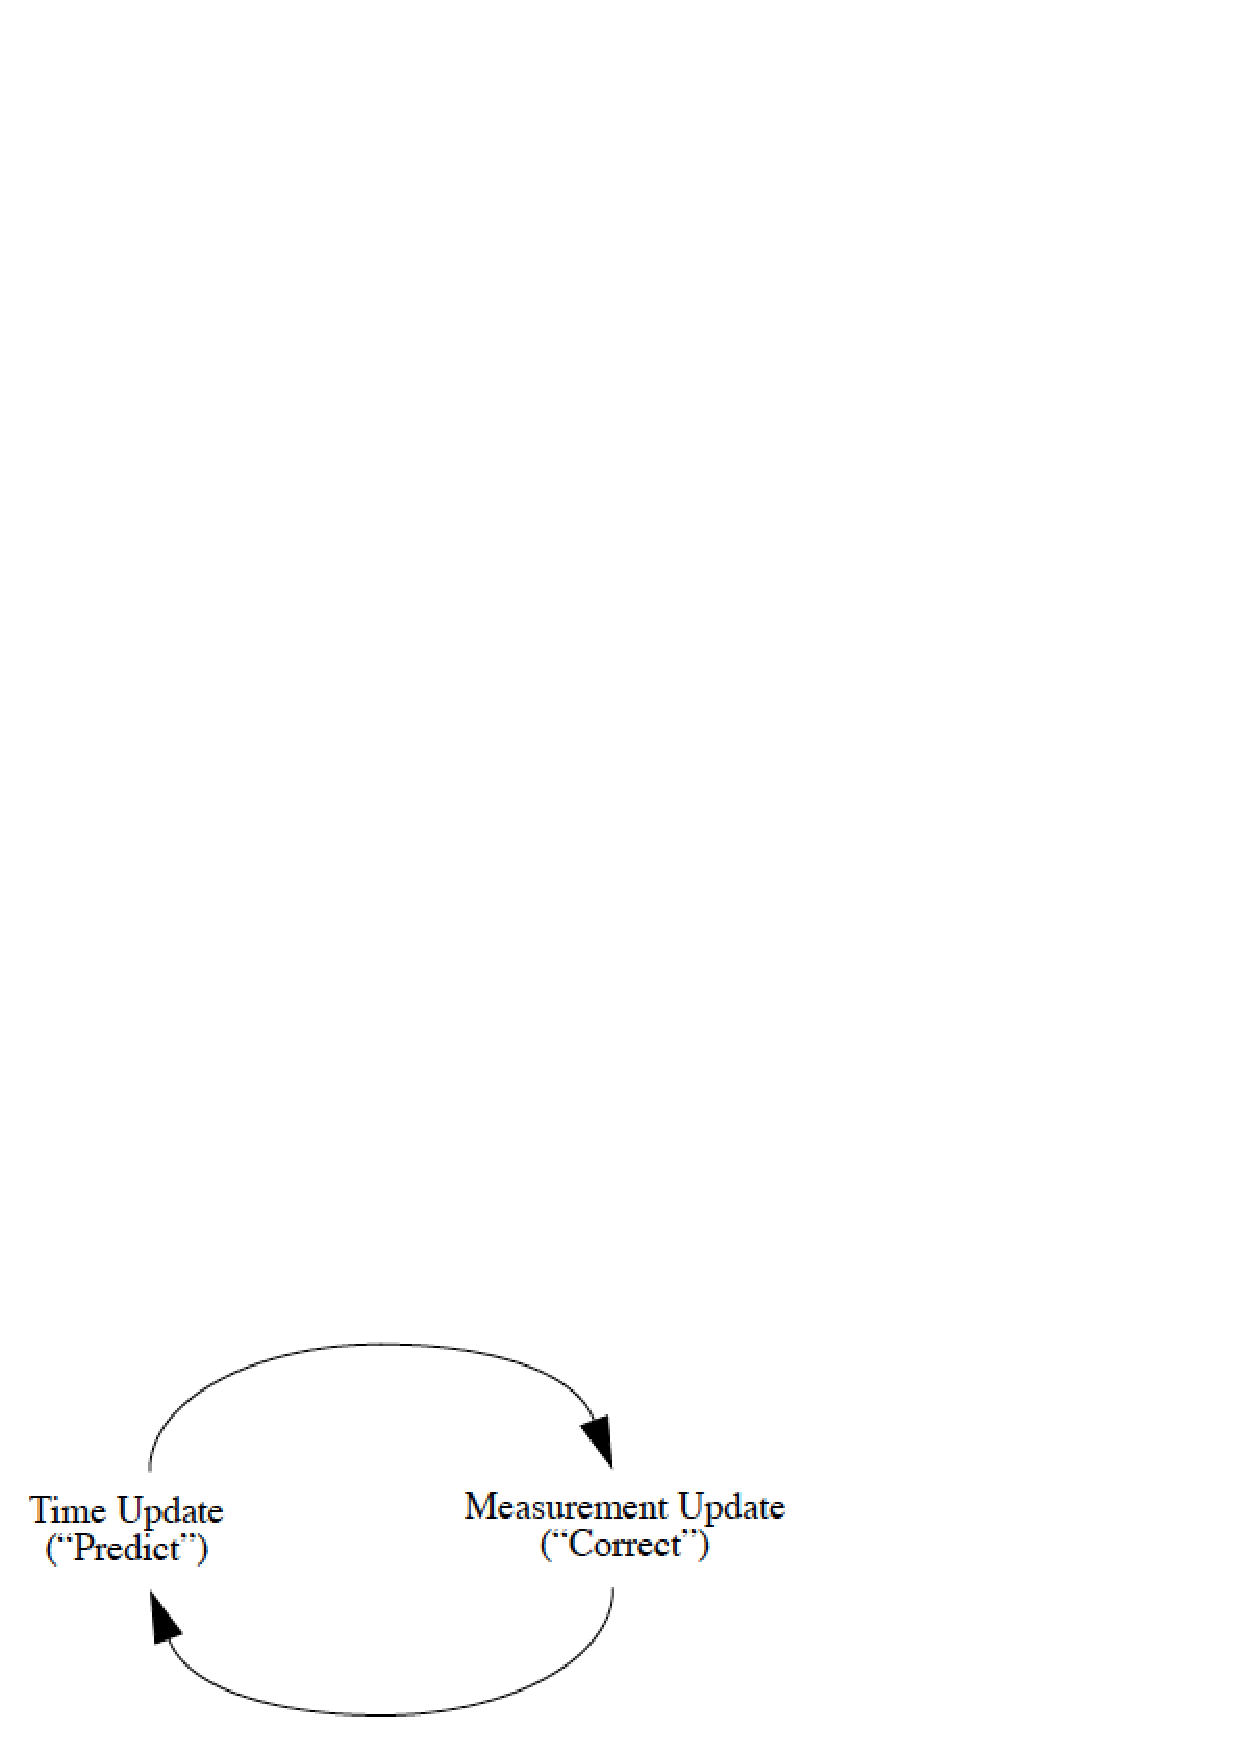
\includegraphics[width=6cm]{pictures/simple_schematic_algo.png}
\caption{A simple structure of the algorithm \cite{welch1997}.}
\label{simple_schematic}
\end{center}
\end{figure}
In a first step the state at $k+1$ is estimated based on \ref{eq1}. This estimation is called a priori state estimation and written as $\hat{x}_k^{-}$. In a second step the a priori state estimation is corrected by the knowledge of measurements $z_k$. This corrected estimation is called the a posteriori estimation and written as $\hat{x}_k$.

Now two errors can be defined with their error covariances. First the error of the a priori estimation 
\begin{equation}
e^{-}=x_k-\hat{x}_k^{-}
\end{equation}
and second the error of the a posteriori estimation 
\begin{equation}
e=x_k-\hat{x}_k
\end{equation}
with the a priori estimate error covariance 
\begin{equation}
P^{-}_k=E[e^{-}e^{-T}]
\end{equation}
and the a posteriori error covariance.
\begin{equation}
P_k=E[ee^{T}]\label{P_post}
\end{equation}

The Kalman Filter is calculating the a posteriori estimation, the one we are finally looking for. This calculation is a linear combination between the a priori estimated state and the difference of the the estimated measurement $x_k*H$ and the actual measurement $z_k$ weighted with the Kalman gain $K$. This difference $z_k-H_k\hat{x}^{-}_k$ is  called residual and tells us how accurate the estimation of the measurements is. This is summarized in equation \ref{eq7}.
\begin{equation}
\hat{x}_k^{-}*K*(z_k-H_k\hat{x}^{-}_k)\label{eq7}
\end{equation}
The Kalman gain $K$ is the heart of the Kalman Filter. $K$, a $n\times n$ Matrix is chosen in a way to minimize the a posteriori error covariance shown in equation \ref{P_post}. With some calculations the following 
\begin{equation}
K=\frac{P^{-}_k*H^{T}_k}{(H_k*P^{-}_k*H^{T}_k+R_k)}
\end{equation}
can be derived for the Kalman gain $K$ \cite{welch1997} 
This concept uses the information of a normal gaussian distribution of the noise mentioned in equations \ref{R_Q_noise}. $P_k$ is minimized using the Maximum Likelihood Estimation and is called the  Gaussian Maximum-Likelihood Estimator. A more detailed derivation of the mathematics is shown in \cite{maybeck1979} and \cite{andrews2007}.

\subsection*{Algorithm}
With the equations described in the section above, the estimation and correction step can be summarized as shown in figure \ref{equation_kalman}.
\begin{figure}[h]
\begin{center}
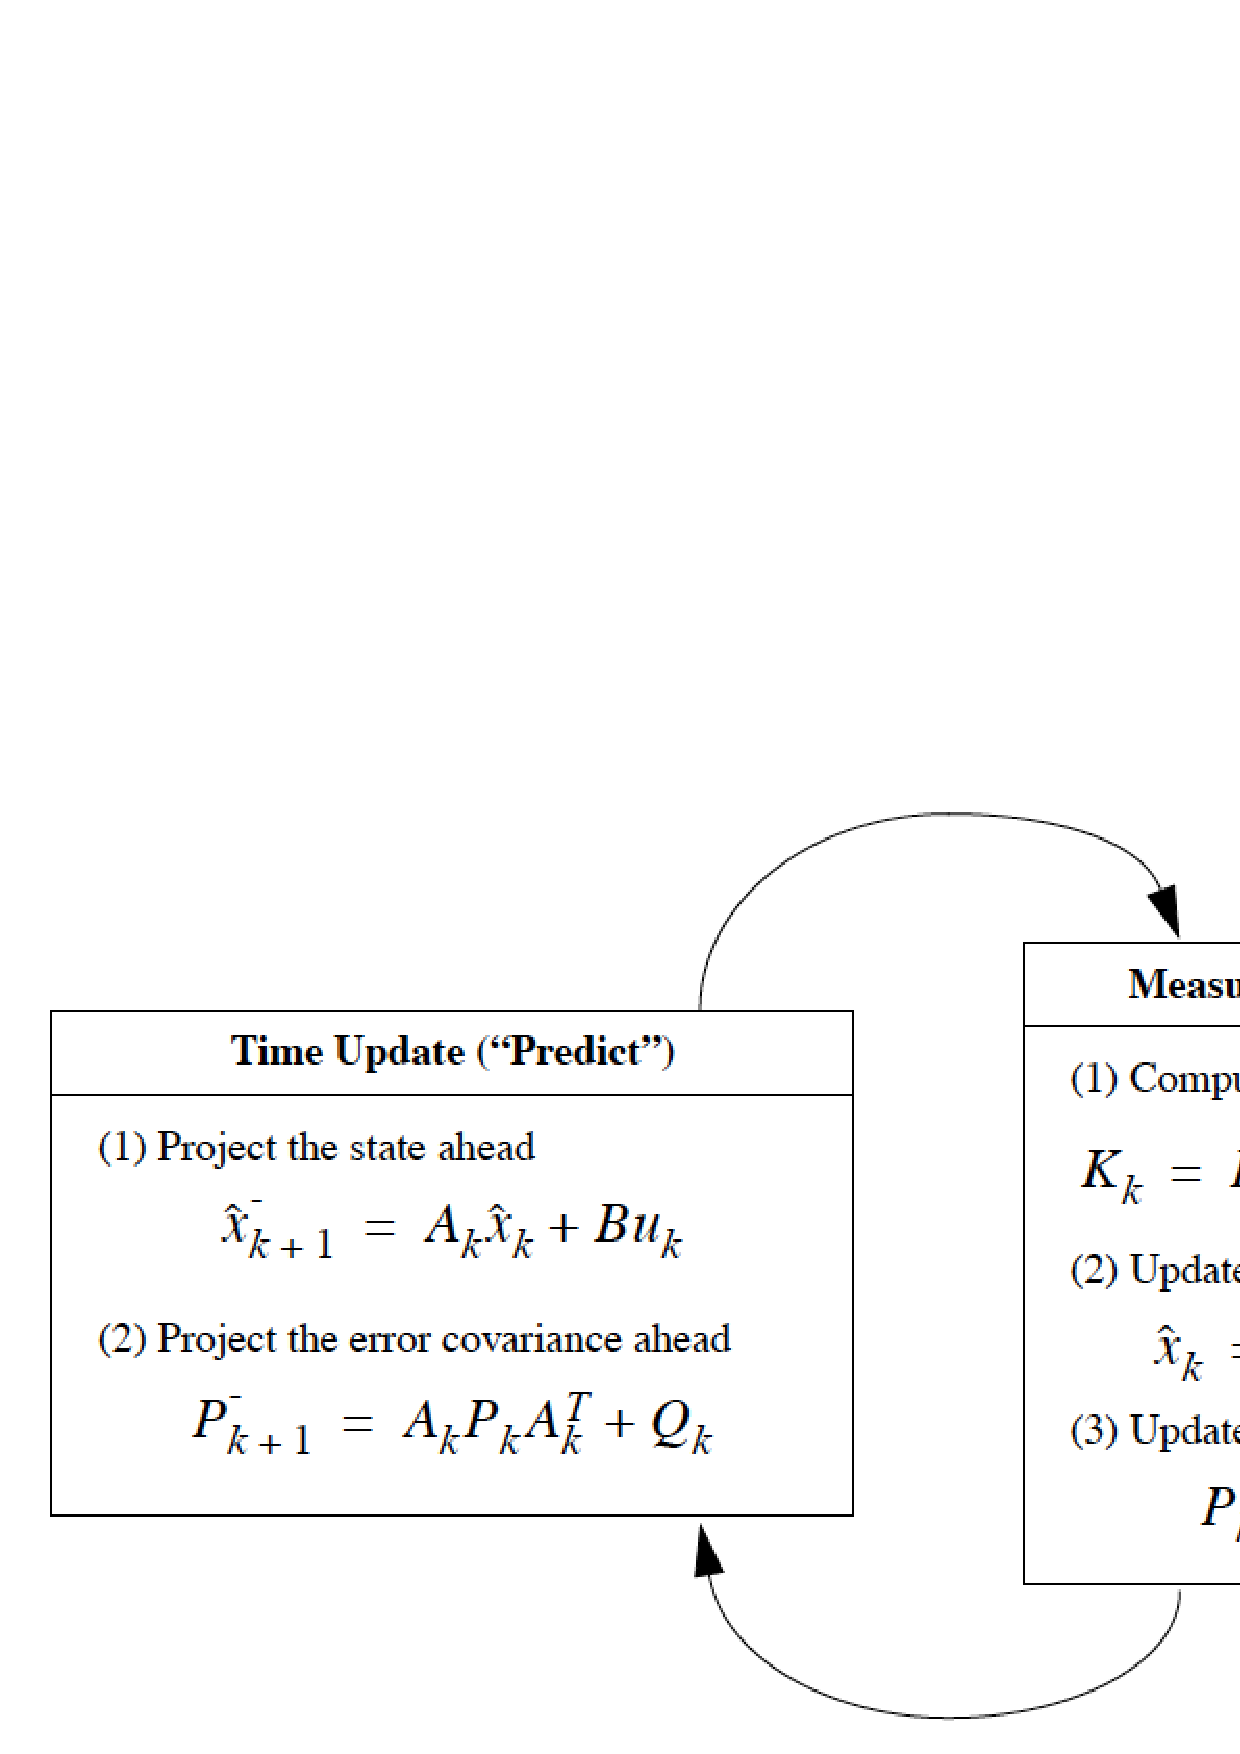
\includegraphics[width=13cm]{pictures/equation_kalman.png}
\caption{The prediction and the correction step with their corresponding equations \cite{welch1997}. }
\label{equation_kalman}
\end{center}
\end{figure} 
For a fine tuning of the filter often the measurement error covariance matrix $R_k$ and process noise $Q_k$ can be used. $R_k$ contains the information how accurate the sensors and therefore the measurements are expected to be. This can be estimated in a first round with some static sensor test or can be found in the data sheets of the sensors. The matrix $Q_k$ describes how correct the propagation model described by the matrix $A_k$ is believed to be. In this sense, the higher one chooses the values and therefore the noise of $R_k$ and $Q_k$ the less influence do the measurements or the propagation model respectively have on the estimated state. Having a diagonal matrix with constant values over time, does not represent the reality, but brings it to a form which is fast stable and easier tunable \cite{welch1997}. 

\subsection*{Extended Kalman Filter (EKF)}\label{ekf}
In reality the process to estimate the new state and the measurement relationship to the process is non-linear.
\begin{equation}
x_{k+1}=f(x_k,u_k,w)
z_k=h(x_k,v_k)
\end{equation}
One of the solution to overcome this problem is the Extended Kalman Filter shortly EKF. The EKF is linearizing the functions with a first order Taylor-Series around the current state. This can be summerized with the following equation:
\begin{equation}
x_{k+1}\approx \hat{x}_{k+1}+A(x_k-\hat{x}_k)+w\\
z_k\approx \hat{z}_k+H(x_k-\hat{x}_k) +v 
\end{equation}
Where $A$ and $H$ are the Jacobian matrix of the function $f$ and $h$.
\begin{equation}
A_{i,j}=\frac{\partial f_{i}}{\partial x_j}(\hat{x}_k,u_k,9)\\
H_{i,j}=\frac{\partial h_{i}}{\partial x_j}(\hat{x}_k,u_k,9)
\end{equation}
This brings us to the summarized equations of the EKF in figure \ref{equation_ekf}. Where W and V are the jaccobians of f() with respect to w and v respectively. But since the models (\ref{state_estimation} and \ref{sensor_estimation} are independent of w and v the derivatives are equal 1.

\begin{figure}[h]
\begin{center}
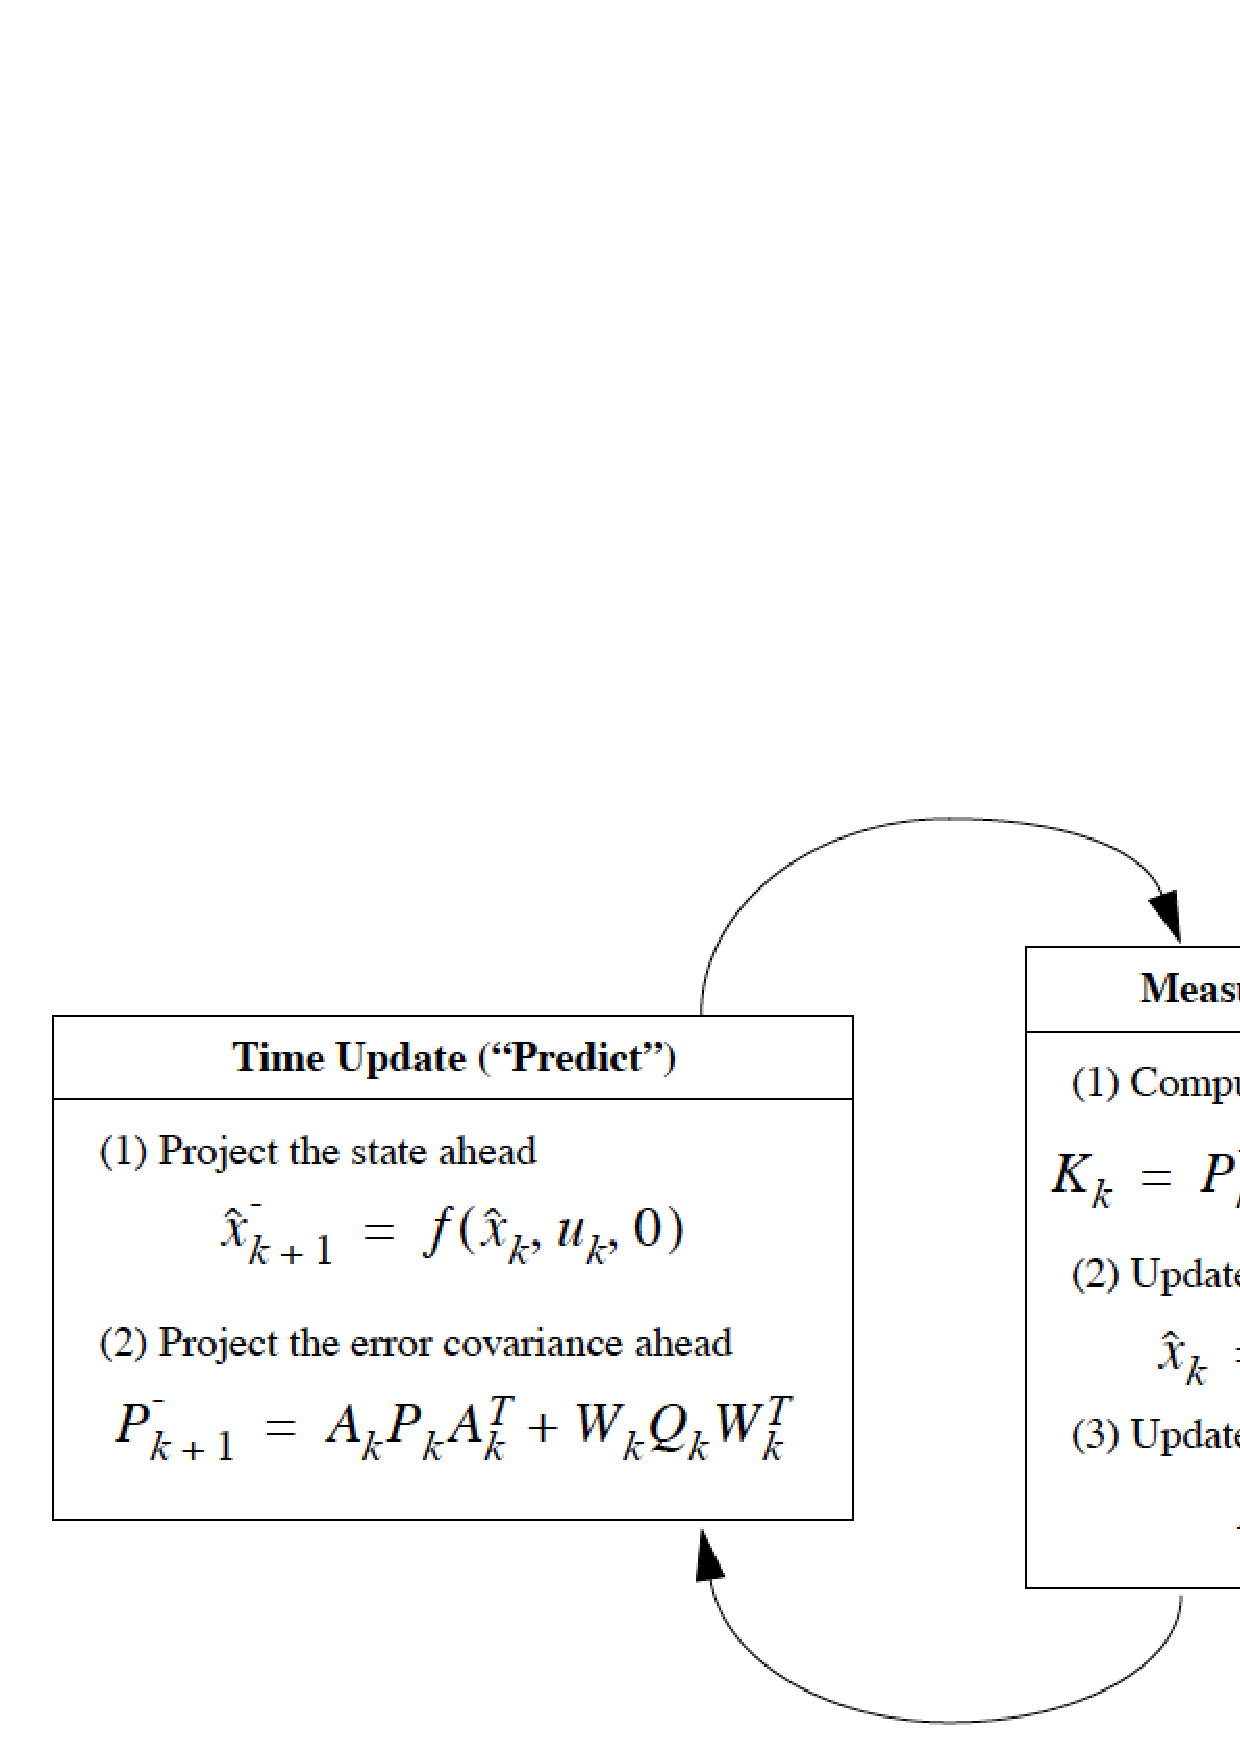
\includegraphics[width=13cm]{pictures/equation_ekf.png}
\caption{The prediction and correction step of the EKF with their corresponding equations \cite{welch1997}. }
\label{equation_ekf}
\end{center}
\end{figure}


\section{Algorithm for State Estimation}
In this chapter we will present the structure of the state estimation algorithm as we implemented it in MATLAB. As mentioned before, the goal is to get an estimation of the system's state as precise as possible using an Extended Kalman Filter. The Algorithm can be split in several main tasks. First the physical relations between the state $x_{k}$ and the state $x_{k+1}$ have to be defined and summarized in a propagation model. This is needed to calculate the a priori state estimation as described in chapter \ref{math_kalman}. Since this step is  crucial for the accuracy of the algorithm, it is further explained in chapter \ref{state_estimation}. A second key role plays the measurement estimation which corrects the a priori state estimation and calculates the a posteriori state estimation. A more detailed explanation of this correction can be found in chapter \ref{sensor_estimation}. A third question to be elaborated is how the algorithm has to behave if no sensor data is available or if not all sensors provide their outputs with the same frequency. In the last paragraph we will explain how the error covariances were chosen.

\subsection*{Orientation}
The estimator algorithm has to handle two different coordinates frames. One is the inertial frame and the other the body frame. The inertial frame is the earth fixed frame. The two measurements position and the velocity both provided by the GPS are in the inertial frame. Also the states of the system are in the inertial frame. The origin of the inertial frame lies at the suspension point of the pendulum/kite. The body frame is a coordinate system on the kite. The propagation model needs the body frame to calculate the forces acting on the body.Measurements form the IMU are as well as in body coordinates since the represent the forces. Its z-axis always points in the direction of the line and its origin lies at the center of gravity of the kite. The sensor measurements from the IMU are all in the body frame. Figure \ref{dof} contains an illustration of these two coordinate systems. 

 \begin{figure}[h]
\begin{center}
\includegraphics[width=10cm]{pictures/sketch_coordinate_systems.png}
\caption{The definition of the inertial and body frame as well as the convention for the angles in the pendulum model.}
\label{dof}
\end{center}
\end{figure}

The euler angles describe how the inertial frame has to be rotated to bring it into the body frame. With other words, the euler angles tell us the orientation of the body frame. With the direct cosine matrix ($DCM$) we can transform a vector from the inertial frame into the body frame and vise versa. For example can the accelerometer data which is given in body frame coordinates be transformed into the inertial frame, where the propagation of the states is calculated \cite{andrews2007}.

\subsection*{Degrees of Freedom}
As stated in the introduction, we implemented two different versions of the state estimation algorithm. A standard implementation assuming a free mass and one version that exploits the constraints given by the knowledge that the mass is oscillatingly suspended at a fixed point. These two versions are quite similar and share a lot of code, but one crucial point where they differ from each other is the number of degrees of freedom (DoF). The free mass model uses 12 DoF, namely position, velocity, attitude and attitude rate. Thus the state vector consists of 12 variables. The pendulum model uses only 6 true degrees of freedom: Three angles representing the position and attitude as well as their respective rates representing velocity and attitude rate. The definition of these angles can be seen in figure \ref{dof}.



\subsection*{States and Measurements}
The state vector in the free mass model with the dimension of 12 looks as follows:
\begin{equation}
 x=
 \begin{pmatrix}
  x \\
  y \\
  z \\
  \dot{x} \\
  \dot{y} \\
  \dot{z} \\
  \phi \\
  \theta \\
  \psi \\
  \dot{\phi} \\
  \dot{\theta} \\
  \dot{\psi} \\
 \end{pmatrix}
\end{equation}
The first six variables are position and velocity in the inertial frame. The angles and angular rates are Euler angles with the convention ZY'X''. This means that in order to get from the inertial frame to the body frame the following three rotations have to be performed: a rotation with angle $\psi$ around the z-axis in the inertial frame, a rotation with angle $\theta$ around the new y-axis and a last rotation with angle $\phi$ around the new x-axis.

The state vector in the pendulum model has eight elements. Even tough only 6 DoF are assumed, two additional variables, the radius and the change in radius, are included in the state to ensure the possibility of loosening the constraint of a fixed line length and implementing a spring model as suggested later on in the outlook section. Thus the state vector is defined as follows:

\begin{equation}
 x=
 \begin{pmatrix}
  \Phi \\
  \Theta \\
  \Psi \\
  r \\
  \dot{\Phi} \\
  \dot{\Theta} \\
  \dot{\Psi} \\
  \dot{r}
 \end{pmatrix}
\end{equation}

For the definition of the angles $\Phi$, $\Theta$ and $\Psi$ see figure \ref{dof}.

 The measurement vector is the same for the free mass model as well as for the pendulum model. It consits of the position (pos) and the velocity (vel) of the GPS, the acceleration (acc) from the accelerometer and the rate of turn (gyro) from the gyroscope and the orientation (mag) from the magnetometer. Each of them in all three dimensions give us the measurement vector z with a dimension of 15.
 
\begin{equation}
 z= \begin{pmatrix}
  pos\;x \\
  pos\;y \\
  pos\;z \\
  vel\;x \\
  vel\;y \\
  vel\;z \\
  acc\;x \\
  acc\;y \\
  acc\;z \\
  gyro\;x \\
  gyro\;y \\
  gyro\;z \\
  mag\;x \\
  mag\;y \\
  mag\;z
 \end{pmatrix}
\end{equation}



\subsection*{Structure of the Algorithm}
In \ref{structure_algo} the schematic of the algorithm is shown. Each of the blocks will now be successively explained.
\begin{figure}
\begin{center}

\includegraphics[width=8 cm]{pictures/structure_aldo_2.png}
\caption{The graphical representation of the algorithm's structure.}

\end{center}
\end{figure}


\begin{description}
\item[Block 1, totalTime:]
The filter estimates with constant rate the state of the system. This rate is independent on any output rate of the sensors. In the first block the time at which the state is estimated is set. It is the old time totalTime added with a constant time step t.

\item[Block 2, Propagation:]
During the second block the a priori state of the system is estimated with the help of the physical model. How and why the physical model is defined is explained in chapter \ref{state_estimation}. After this step the vector $x_{est}$ is up to date.

\item[Block 3, Finding newest Data:]
If there is no new data available until the time of the a priori estimated state, the correction step is not executed. This allows the algorithm to run the EKF with a higher rate, then the IMU and GPS provide data. If there is new data available, the algorithm is finding the newest or closest one to the a priori estimation time (totalTime). To summarize: If we have no new data from the sensors the system just keeps propagating based on the physical model. If there is at least one new measurement from any sensor block 4 will be executed.If we have new data, the algorithm takes the newest one for the correction.

\item[Block 4, measurement selection:]
Not all sensors of an IMU provide an output with the same rate. Here it is tested, which sensors actually have a new output value and which has still it's output value from the previous dataset. The correction step in block 5 is only executed for measurements with new data and therefore only these have an influence updating the a priori estimation to the a posteriori estimation.

\item[Block 5, correction:]
As last step the correction of the a priori estimation takes place and the posteriori estimation is calculated. How the relationship between the state and the measurements look like is explained in chapter \ref{sensor_estimation}
\end{description}


\subsection*{Error Covariance}
For the measurement error covariance the noise of the different sensors are taken from the data sheets. But they were manually scaled according to have more accurate and stable filter. For the propagation model the covariance was estimated on how accurate the equations are. But also in this case were they manually adjusted afterwards. For an easier handling only the diagonal elements have a value. The off diagonal values are all zero.

\subsection*{Jacobian Matrix}
In chapter \ref{ekf} the matrixes H and A were derived. Since the physical model and relations between state and the measurements are non linear, H and A are the Jacobian matrixes of the functions $f$ and $h$. For having an accurate as possible solution the Jacobian was in a first version calculated analytically with symbolic toolbox from MathWorks. The Jacobian matrix then has to be evaluated in every iteration step. Simulating 0.01 seconds took the filter much longer than 10 minutes. It was then decided to rewrite the algorithm calculating the Jacobian matrixes numerical. The function ekf.m \cite{mcekf} from MathWorks was restructured to match the requirements of this algorithm. It uses a complex step differentiation to calculate the derivatives of the function f and h \cite{diehl11}. 


\section{State Estimation Model}\label{state_estimation}
In order to propagate the state of the system $x_{k}$ to the a priori state estimation $x^{-}_{k+1}$ the filter needs to be able to predict in what state the system will be at time $t_{k+1}$ based on its state at time $t_{k}$ and the control inputs, if there are any. In the most basic case, the assumption is that there exists no knowledge about the forces acting on the body. This leads to the so called "free mass model". However, in the case of a kite tethered to a ground station, the body is not able to move freely in three dimensions, but its movement is in a first approximation limited to a sphere with a given radius. This means, that one of the main forces acting on the body, the centripedal force, can be accounted for in the prediction. Furthermore an aerodynamical model of the kite might be able to predict also other forces than the centripedal force. In order to explore the benefits of such a model, we decided to use a spherical pendulum for the reasons described in the introduction. In that case, all the forces acting on the body are known and the degrees of freedom are further reduced due to the bridled suspension. In the following sections, these two models are going to be described in detail. 

\subsection*{Free Mass Model}
The dynamics of the body are described by a system of first order differential equations describing the change in the state variables.
\begin{equation} \dot{x}=g(x,t)  \end{equation}
In this case the model is time invariant and thus g is not time dependent. 
\begin{equation} \dot{x}=g(x)  \end{equation}
Since there is no knwoledge about the forces acting on the body, this set of equation looks rather simple: 
\begin{equation} g(x)=\begin{bmatrix}  x_{4} \\  x_{5} \\ x_{6} \\ 0 \\ 0 \\ 0 \\ x_{10} \\ x_{11} \\ x_{12} \\ 0 \\ 0 \\0 \end{bmatrix} \end{equation}

\subsection*{Pendulum}
Again the dynamics are described by a system of time invariant first order differential equations. 
\begin{equation} \dot{x}=g(x)  \end{equation}
Due to the gravitation and the centripedal force being the only forces acting on the body, we can derive an exact set of differential equations that govern the motion of a spherical pendulum. Therefore we use the Euler-Lagrange-Equation to derive the differential equations as suggested in \cite[156ff]{debnath2005}.

With the kinetic energy
\begin{equation} T=\frac{1}{2}mr^2(\dot{\Theta}^2+\dot{\Psi}^2\cos^2{\Theta})  \end{equation}
and the potential energy
\begin{equation} V=-mr\sin{\Theta}  \end{equation}
the Lagrangian is defined by:
\begin{equation} L=T-V = \frac{1}{2}mr^2(\dot{\Theta}^2+\dot{\Psi}^2\cos^2{\Theta})+mr\sin{\Theta}\end{equation}

Substituting the Lagrangian into Euler-Lagrange-Equation 
\begin{equation} \frac{\partial L}{\partial \Psi}-\frac{d}{dt}\frac{\partial L}{\partial \dot{\Psi}}=0 \end{equation}
and solving for $\ddot{\Psi}$ results in:
\begin{equation} \ddot{\Psi}=2\tan{\Theta}\dot{\Theta}\dot{\Psi} \end{equation}

And similarly for $\ddot{\Theta}$:
\begin{eqnarray} \frac{\partial L}{\partial \Theta}-\frac{d}{dt}\frac{\partial L}{\partial \dot{\Theta}}=0 \\
 \ddot{\Theta}=\dfrac{\cos{\Theta}(g-r\sin{\Theta}\dot{\Psi}^2)}{r} \end{eqnarray}

The third degree of freedom, the body's rotation about its z-axis, is assumed to be constant. However, due to the convention of the euler angles, a change in phi contributes an additional term to the z component of the rotation vector in the body frame. (As can be seen in equation \ref{deuler2body}) To compensate for that, the second derivative of $\Phi$ is not zero but defined as follows: 

\begin{eqnarray} \frac{d}{dt}w_{z}^{body}=\frac{d}{dt}(\dot{\Phi} - \sin{\Theta} \dot{\Psi}) =0 \\
 \ddot{\Phi}=\cos{\Theta}\dot{\Theta}\dot{\Psi}+\sin{\Theta}\ddot{\Psi} \end{eqnarray}

With the radius assumed to be constant, the fourth and eighth state variable ($r$ and $\dot{r}$) are not changing and thus their time derivatives are zero.

Therefore the set of differential equations is given by:
\begin{equation} g(x)=\begin{bmatrix} \\ x_{5} \\ x_{6} \\ x_{7} \\ 0 \\ \cos{x_{2}} \dot{x_{2}} \dot{x_{3}}+\sin{x_{2}} \ddot{x_{3}} \\  \dfrac{\cos{x_{2}}(g-r\sin{x_{2}} \dot{x_{3}}^2)}{r} \\ 2\tan{x_{2}} \dot{x_{2}} \dot{x_{3}} \\ 0  \end{bmatrix} \end{equation}

\subsection*{Solving the Differential Equations}
So far we have derived the sets of differential equations that contain all the knowledge we have about the systems. To calculate the a priori state estimation $x^{-}_{k+1}$ from the state of the system $x_{k}$ we now only need to solve these sets of differnetial equations. This is done numerically using the classical fourth-order Runge-Kutta method \cite{Kutta1901}.\footnote{This is the same method that is used in Matlab's built in ODE45 differential equation solver, with the difference that it only uses one timestep. This leaves the possibility to analytically derive the Jacobian matrix.} Note that in our case g(x) is time invariant. 
\begin{eqnarray}k_{1}&=&h g(t_{n},x_{n})\\
k_{2}&=&h g(t_{n}+\frac{1}{2}h,x_{n}+\frac{1}{2}k_{1})\\
k_{3}&=&h g(t_{n}+\frac{1}{2}h,x_{n}+\frac{1}{2}k_{2})\\
k_{4}&=&h g(t_{n}+h,x_{n}+k_{3})\\
x_{n+1}&=&x_{n} + \frac{1}{6} k_{1} + \frac{1}{3} k_{2} + \frac{1}{3} k_{3} + \frac{1}{6} k_{4} + \mathcal{O}(h^{5})\end{eqnarray}

\section{Sensor Estimation Model}\label{sensor_estimation}
An illustration of the relation between the position and velocity in $(y,x,z)$ or $(dx,dy,dz)$ and the two angles $\Phi$, $\Theta$ and $\Psi$  is shown in figure \ref{dof}. With this sketch, the assumption of a constant radius and the fact that the velocity is the derivative of the position we get to the equations: 

\begin{eqnarray}
pos\;x&=&R*cos(\Theta)cos(\Psi)\\
pos\;y&=&R*sin(\Psi)cos(\Theta)\\
pos\;z&=&R*sin(\Theta)\\
vel\;x&=&-sin(\Theta)cos(\Psi)*R*\dot{\Theta}-cos(\Theta)sin(\Psi)*R*\dot{\Psi}\\
vel\;y&=&-sin(\Theta)sin(\Psi)*R*\dot{\Theta}+cos(\Theta)cos(\Psi)*R*\dot{\Psi}\\
vel\;z&=&-cos(\Theta)*R*\dot{\Theta}\\
\end{eqnarray}
The centripetal acceleration always acting in z direction of the sensor can be calculated by the formula:
\begin{equation}
a_{cp}=\frac{v^2}{R}
\end{equation}
We then have the an additional acceleration of the earth gravitation. The earth gravitation is in the inertial frame only in z direction and has to be transformed with the $DCM_{bi}$ from the inertial in the body frame. However, since the accelerometer is suspended in a pendulum, it will only measure a z component. The component of g tangential to the sphere, will just accelerate the box and thus not show up in the measurements. Finally the acceleration can be written as:
\begin{equation}
acc= \begin{bmatrix} 0\\0\\ \frac{v^2}{R}\end{bmatrix}+\begin{bmatrix}0\\0\\cos(\Theta) g\end{bmatrix}
\end{equation}
The magnetic field is  a constant value in Zurich. By transforming that into the body frame again with the help of the $DCM_{bi}$, the expected measurement from the magnetometer is calculated:
\begin{equation}
mag= DCM_{bi}* \begin{bmatrix} 0.2145 \\ 0.0060 \\ 0.4268 \end{bmatrix} [gauss]
\end{equation} 
The gyroscope measurement is directly represented by the rate of the euler angles $\dot{\Phi}$,$\dot{\Theta}$ and $\dot{\Psi}$. Since the euler angular rate has to be transformed into the body frame coordinates and additinally has a converstion about which axes is rotated the first, what the gyroscope has not,a transformation matrix has to be used as follows:
\begin{equation}\label{deuler2body}
gyro=\begin{bmatrix} 1 & 0 & -sin(\Theta) \\ 0 & cos(\Phi) & sin(\Phi) cos(\Theta) \\ 0 & -sin(\Phi) & cos(\Phi)cos(\Theta) \end{bmatrix}*\begin{bmatrix} \dot{\Psi}\\ \dot{\Theta}\\ \dot{\Phi} \end{bmatrix}
\end{equation}
Because the position of the senors is not at the center of mass of the pendulum, an additional displacement vector has to be added to the position (compare figure \ref{displacement}). With transforming the distance between the center of mass and the sensor into the inertial frame, the position is adjusted. The displacement gives an additional velocity which is the crossproduct of the rate of rotation and the displacement from the center of mass. By the derivative of this additional velocity the additional acceleration is calculated. The displcement has no influence on the gyrometer measurement and the magnetometer.
\begin{figure}[h]
\begin{center}
\includegraphics[width=8 cm]{pictures/displacement_2.png}
\caption{The black dot represents the sensor, while r is the distance between the center of mass of the pendulum and the sensor.}
\label{displacement}
\end{center}
\end{figure}


\clear
    \chapter{Results - Vicon Test}\label{cha4}
\section{Set up}
\section{Evaluation}
\subsection{short vs long radius}
\subsection{Outage and Sensor rate}
\subsection{Pixhawk vs Xsens}



\clear
    \chapter{Conclusion and Outlook}\label{cha}
\section{Sensor Selection}
The centrifuge test was not able to give a meaningful conclusion about the quality of the different sensors. There seems to be a correlation between the acceleration acting on the sensors and their accuracy, but this could also be due to more vibrations at higher speeds. However, the test showed some general limitations in the range of the different IMU's. The PX4 was not able to cover the whole acceleration range and the MTi-G could not measure rates of turn larger than 403 deg/s. In order to be able to better compare these different units, a test would have to be done where a precise ground truth would be available. Furthermore, the MTi-G should be set to output the calibrated measurements, as this spares the conversion to conventional units.

\section{State Estimation}
Based on the Vicon test, we were able to show an improvement of accuracy in the state estimation when using the "pendulum model"-estimator. Especially in the absence of a GPS signal, this algorithm was still able to estimate the true position while the conventional Kalman Filter drifted off during such periods. This improvement is on one hand due to the reduction in degrees of freedom, giving more redundant measurements per state, and on the other hand due to the accurate prediction of the future states by using the exact knwoledge of the forces acting on the body. These promising results make us confident, that position estimation of a kite with an Extended Kalman Filter could be improved by including as much knowledge of the system as possible. The complete independence of the GPS measurements in the pendulum case, suggests that also in the more complex system of the kite, the dependency on an accurate GPS signal could be reduced.

For future investigations in this subject, we suggest to also investigate the use of models with 8 or more degrees of freedom, allowing for example the radius to vary. Furthermore, the ideal combination of Covariance matrices would have to be found either by finding the exact uncertainties in the sensors and the prediction, or by minimizing the output error. Considering the application of the algorithm to kites, it would be interesting to find out how sensitive the filter is to errors in the prediction of the forces acting on the body. If an very accurate propagation model, as the one of the pendulm that was used in this work, is needed, the algorithms application to a real kite system could prove to be difficult since these systems are a lot more complex. However, investigating the use of additional sesors, like for example line angle sensors, the possibilities of an exact estimation of the kites position and orientation without relying on a GPS signal could be determined. 

\clear
    %\include{Zusammenfassung}
\clear
    %\include{Ausblick}
\clear
    %Bibliography
    \bibliographystyle{unsrt}
    \bibliography{bibliography}
\clear
%\begin{appendix}
    %Appendix
    \appendix
    \chapter{Data Sheets of the PX4 sensors}\label{ds}
\section{Data Sheet of the Accelerometer}\label{ds_acc}
\includepdf[pages=1]{appendix/acc-BST-BMA180-FL000-03.pdf}
\section{Data Sheet of the Gyroscope}\label{ds_gyro}
\includepdf[pages=9]{appendix/gyro_px4.pdf}
\section{Data Sheet of the Magnetometer}\label{ds_mag}
\includepdf[pages=2]{appendix/mag_px4.pdf}
\chapter{Data Sheets of the x-IMU sensors}\label{ds_ximu}
\section{Data Sheet of the Gyroscope}
\includepdf[pages=8]{appendix/x-imu_gyro.pdf}
\section{Data Sheet of the Accelerometer and Magnetometer}
\includepdf[pages=11]{appendix/x-imu_acc_mag.pdf}


    % uncomment the following line in case you need to make the page wider
    %\addtolength{\headwidth}{1.2cm}\addtolength{\textwidth}{0.5cm}
    %\include{Schematics}
%\end{appendix}
\clear
    %%%%\include{Software}
    % uncomment the following line in case you made the page wider earlier
    %\addtolength{\headwidth}{-1.2cm}\addtolength{\textwidth}{-0.5cm}

\end{document}
